\documentclass[aspectratio=169,9pt]{beamer}

\usepackage{graphicx,caption,subcaption,hyperref,amsmath,tikz}
\graphicspath{ {./figures/} }
\captionsetup{font=scriptsize,labelfont=scriptsize}
\setbeamerfont{footnote}{size=\scriptsize}
\usepackage[strict]{changepage}
\usetikzlibrary{arrows,automata,positioning}
\usetheme[titleformat=smallcaps,
            sectionpage=progressbar,
			subsectionpage=progressbar,
			progressbar=frametitle,
			numbering=fraction]{metropolis}
% \usecolortheme{owl}
\usepackage[style=apa,
			sorting=nyt,
			date=year,
			bibencoding=utf8,
			isbn=false,
			eprint=false,
			dashed=false,
			uniquelist=false,
			maxbibnames=2,
			minbibnames=1,
			maxcitenames=2,
			uniquename=init,
			giveninits=true,
			useprefix=false,
			minsortnames=1,
			maxsortnames=2]{biblatex}
\bibliography{References}

% Information to be included in the title page:
\title{4 states $\neq$ 4 dimensions: ProNeural-Mesenchymal antagonism dominates the patterns of phenotypic heterogeneity in Glioblastoma}
\subtitle{CSB Lab Symposium}

\author{Harshavardhan BV \\ {\small Advisors: Mohit Kumar Jolly (BE), Srimonta Gayen (DBG)}}
\date{October 19, 2023}
\institute{IMI, IISc Bangalore}

\begin{document}
    \frame{\titlepage}
%     \section{Introduction}

    \begin{frame}{Glioblastoma Multiforme(GBM)}
    \begin{adjustwidth}{-5cm}{-5cm}
            \centering
            \begin{figure}
                \centering
                \begin{subfigure}{0.35\textwidth}
                    \centering
                    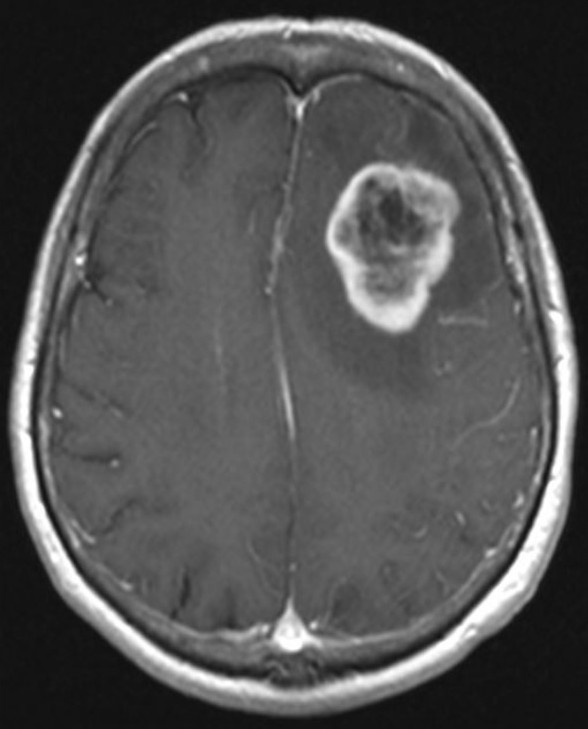
\includegraphics[width=\textwidth]{GBM}
                    \caption{MRI image of Glioblastoma \footnotemark[1]}
                \end{subfigure}
                \pause
                \begin{subfigure}{0.25\textwidth}
                    \centering
                    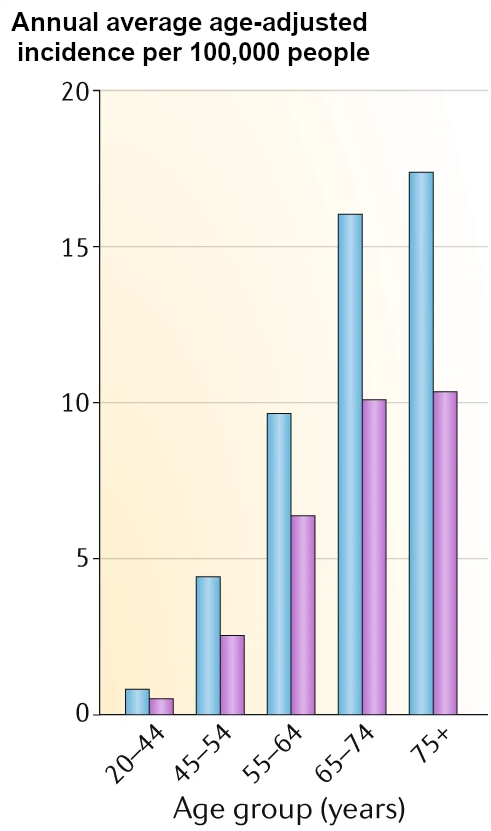
\includegraphics[width=\textwidth]{GBMincid}
                    \caption{Incidence statistics for GBM \footnotemark[2]}
                \end{subfigure}
                \begin{subfigure}{0.25\textwidth}
                    \centering
                    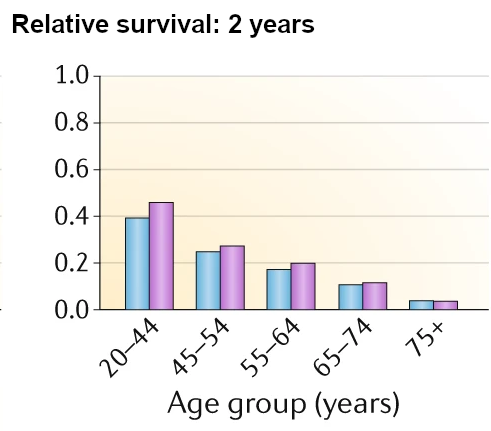
\includegraphics[width=\textwidth]{GBMsurv}
                    \caption{Survival statistics for GBM \footnotemark[2]}
                \end{subfigure}
            \end{figure}
            \footnotetext[1]{\cite{tan}}
            \footnotetext[2]{\cite{molinaro}}
        \end{adjustwidth}
    \end{frame}

    \begin{frame}{Molecular subtypes of GBM}
        \begin{adjustwidth}{-5cm}{-5cm}
            \centering
            \begin{figure}
                \centering
                \begin{subfigure}{0.6\textwidth}
                    \centering
                    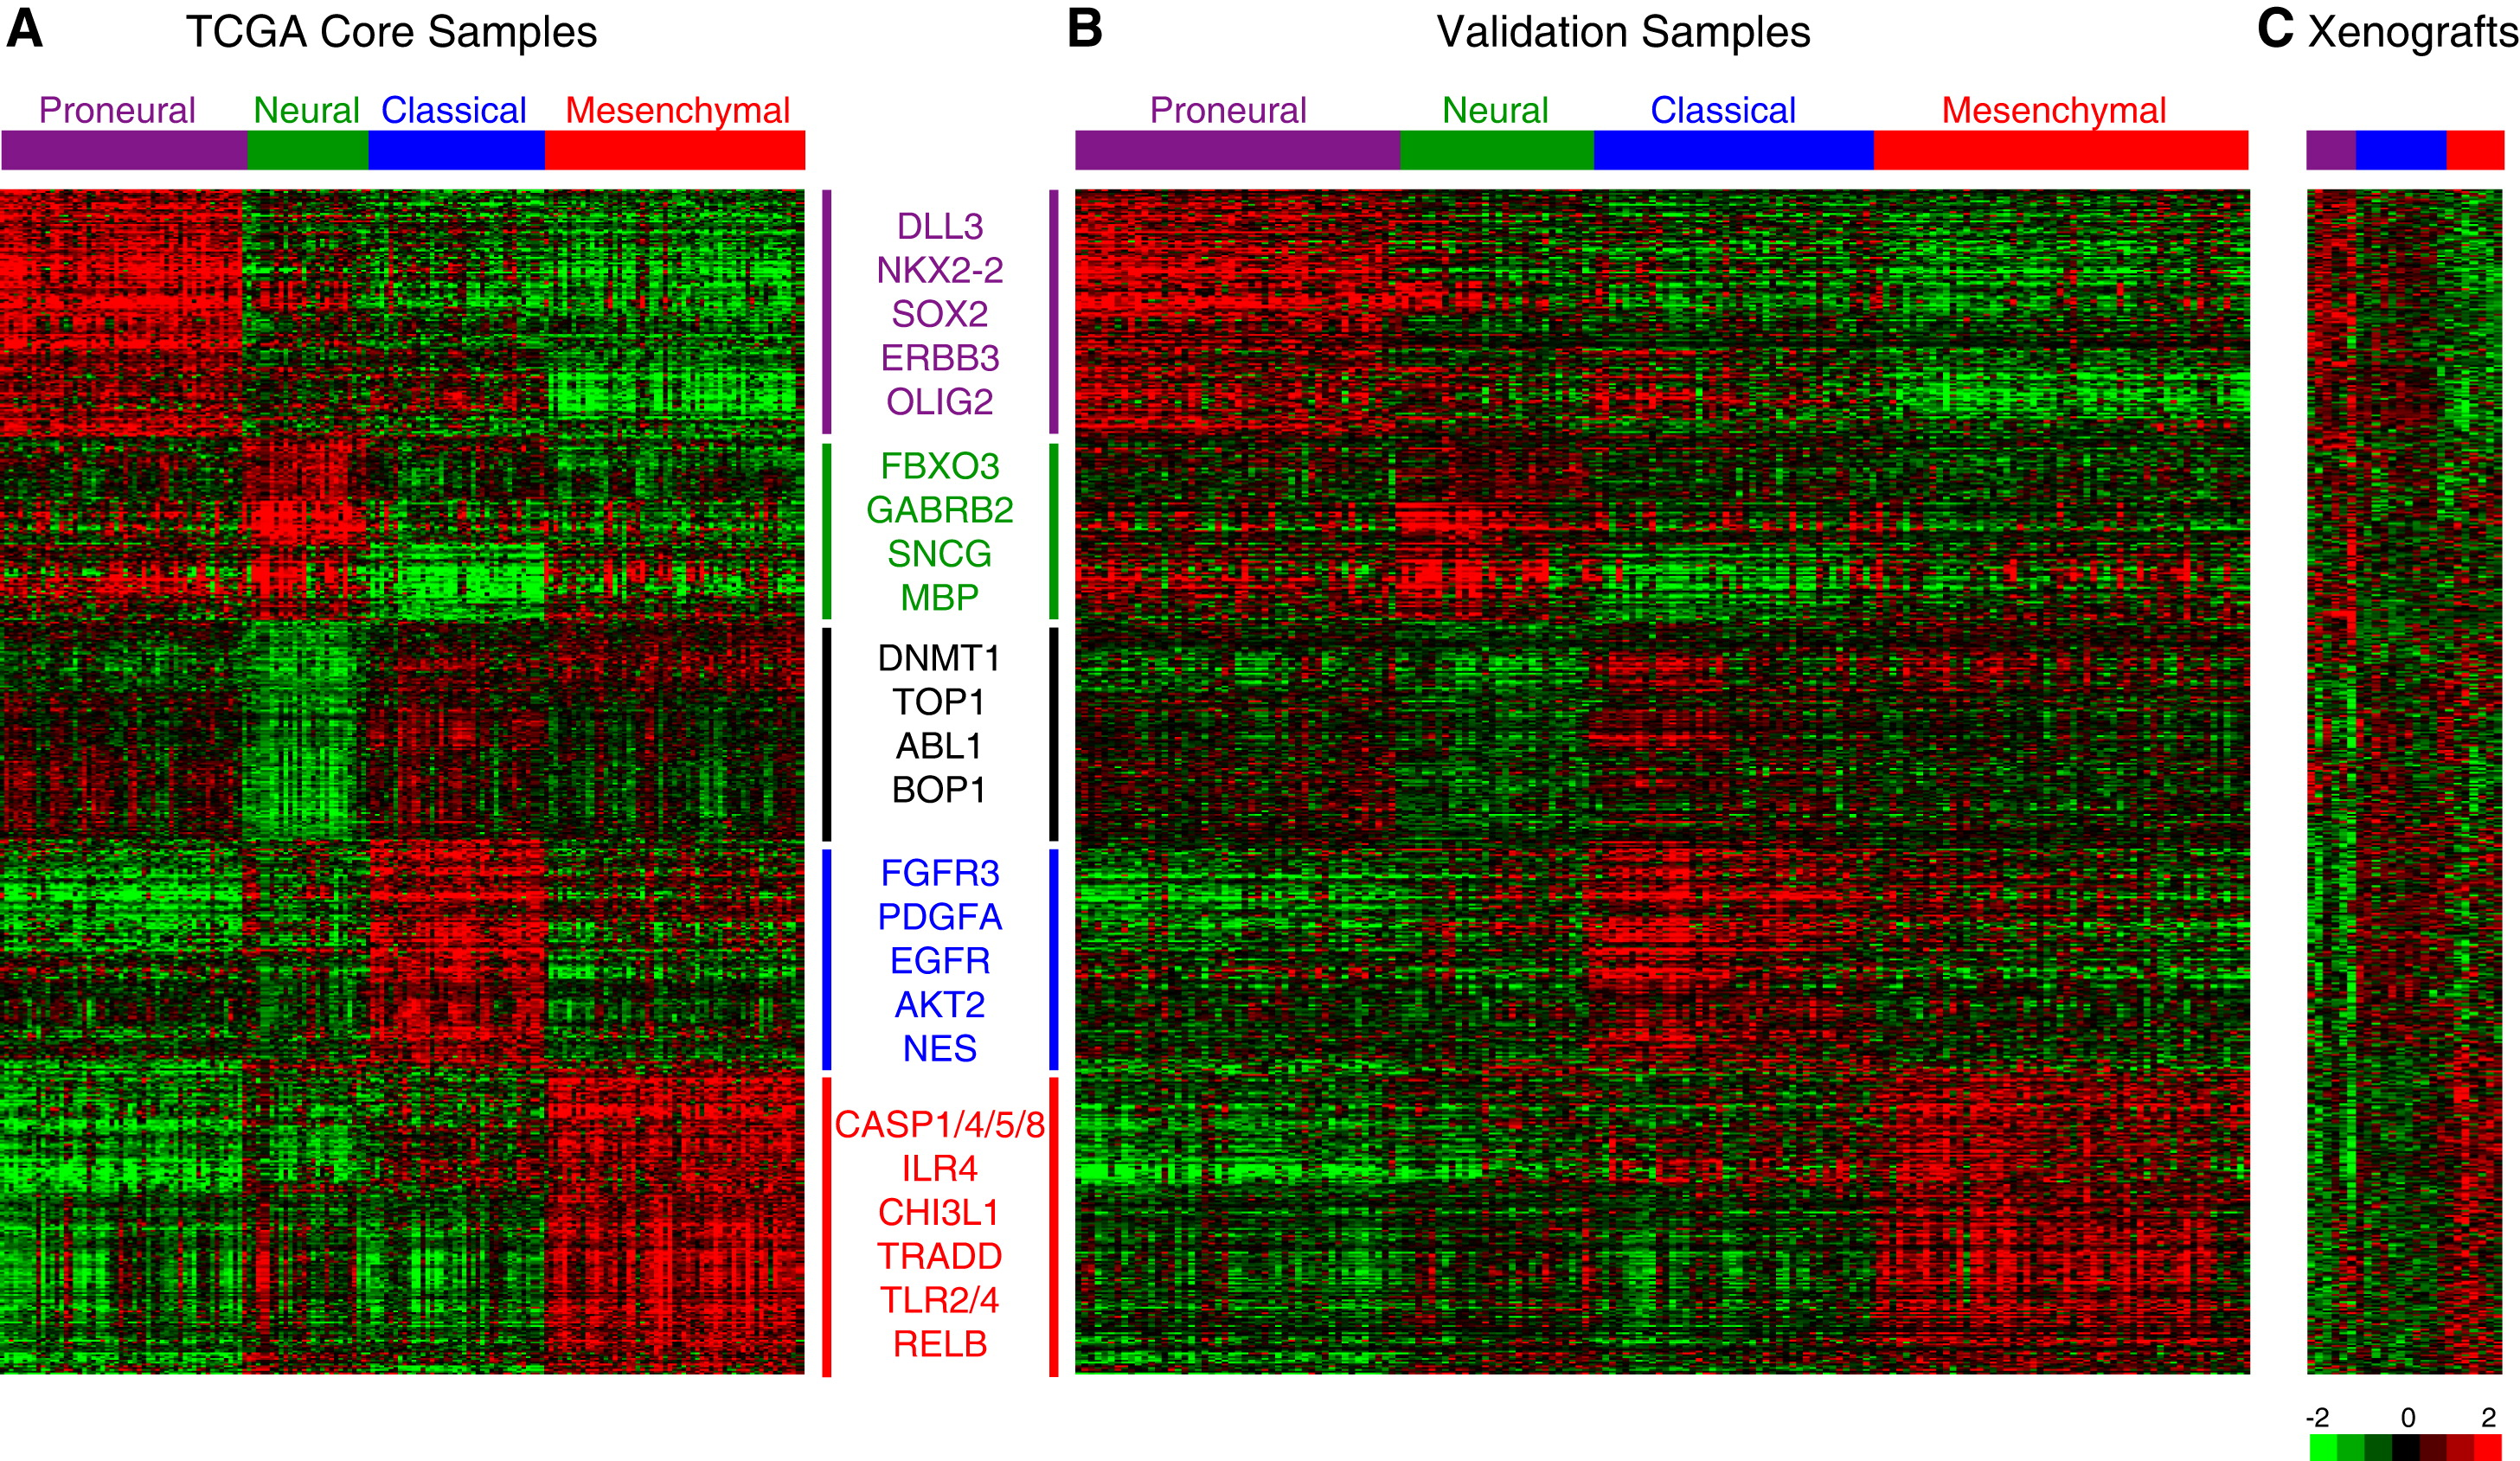
\includegraphics[width=\textwidth]{verhaak_clusters}
                    \caption{Cell states by \cite{Verhaak}}
                \end{subfigure}
                \pause
                \begin{subfigure}{0.4\textwidth}
                    \centering
                    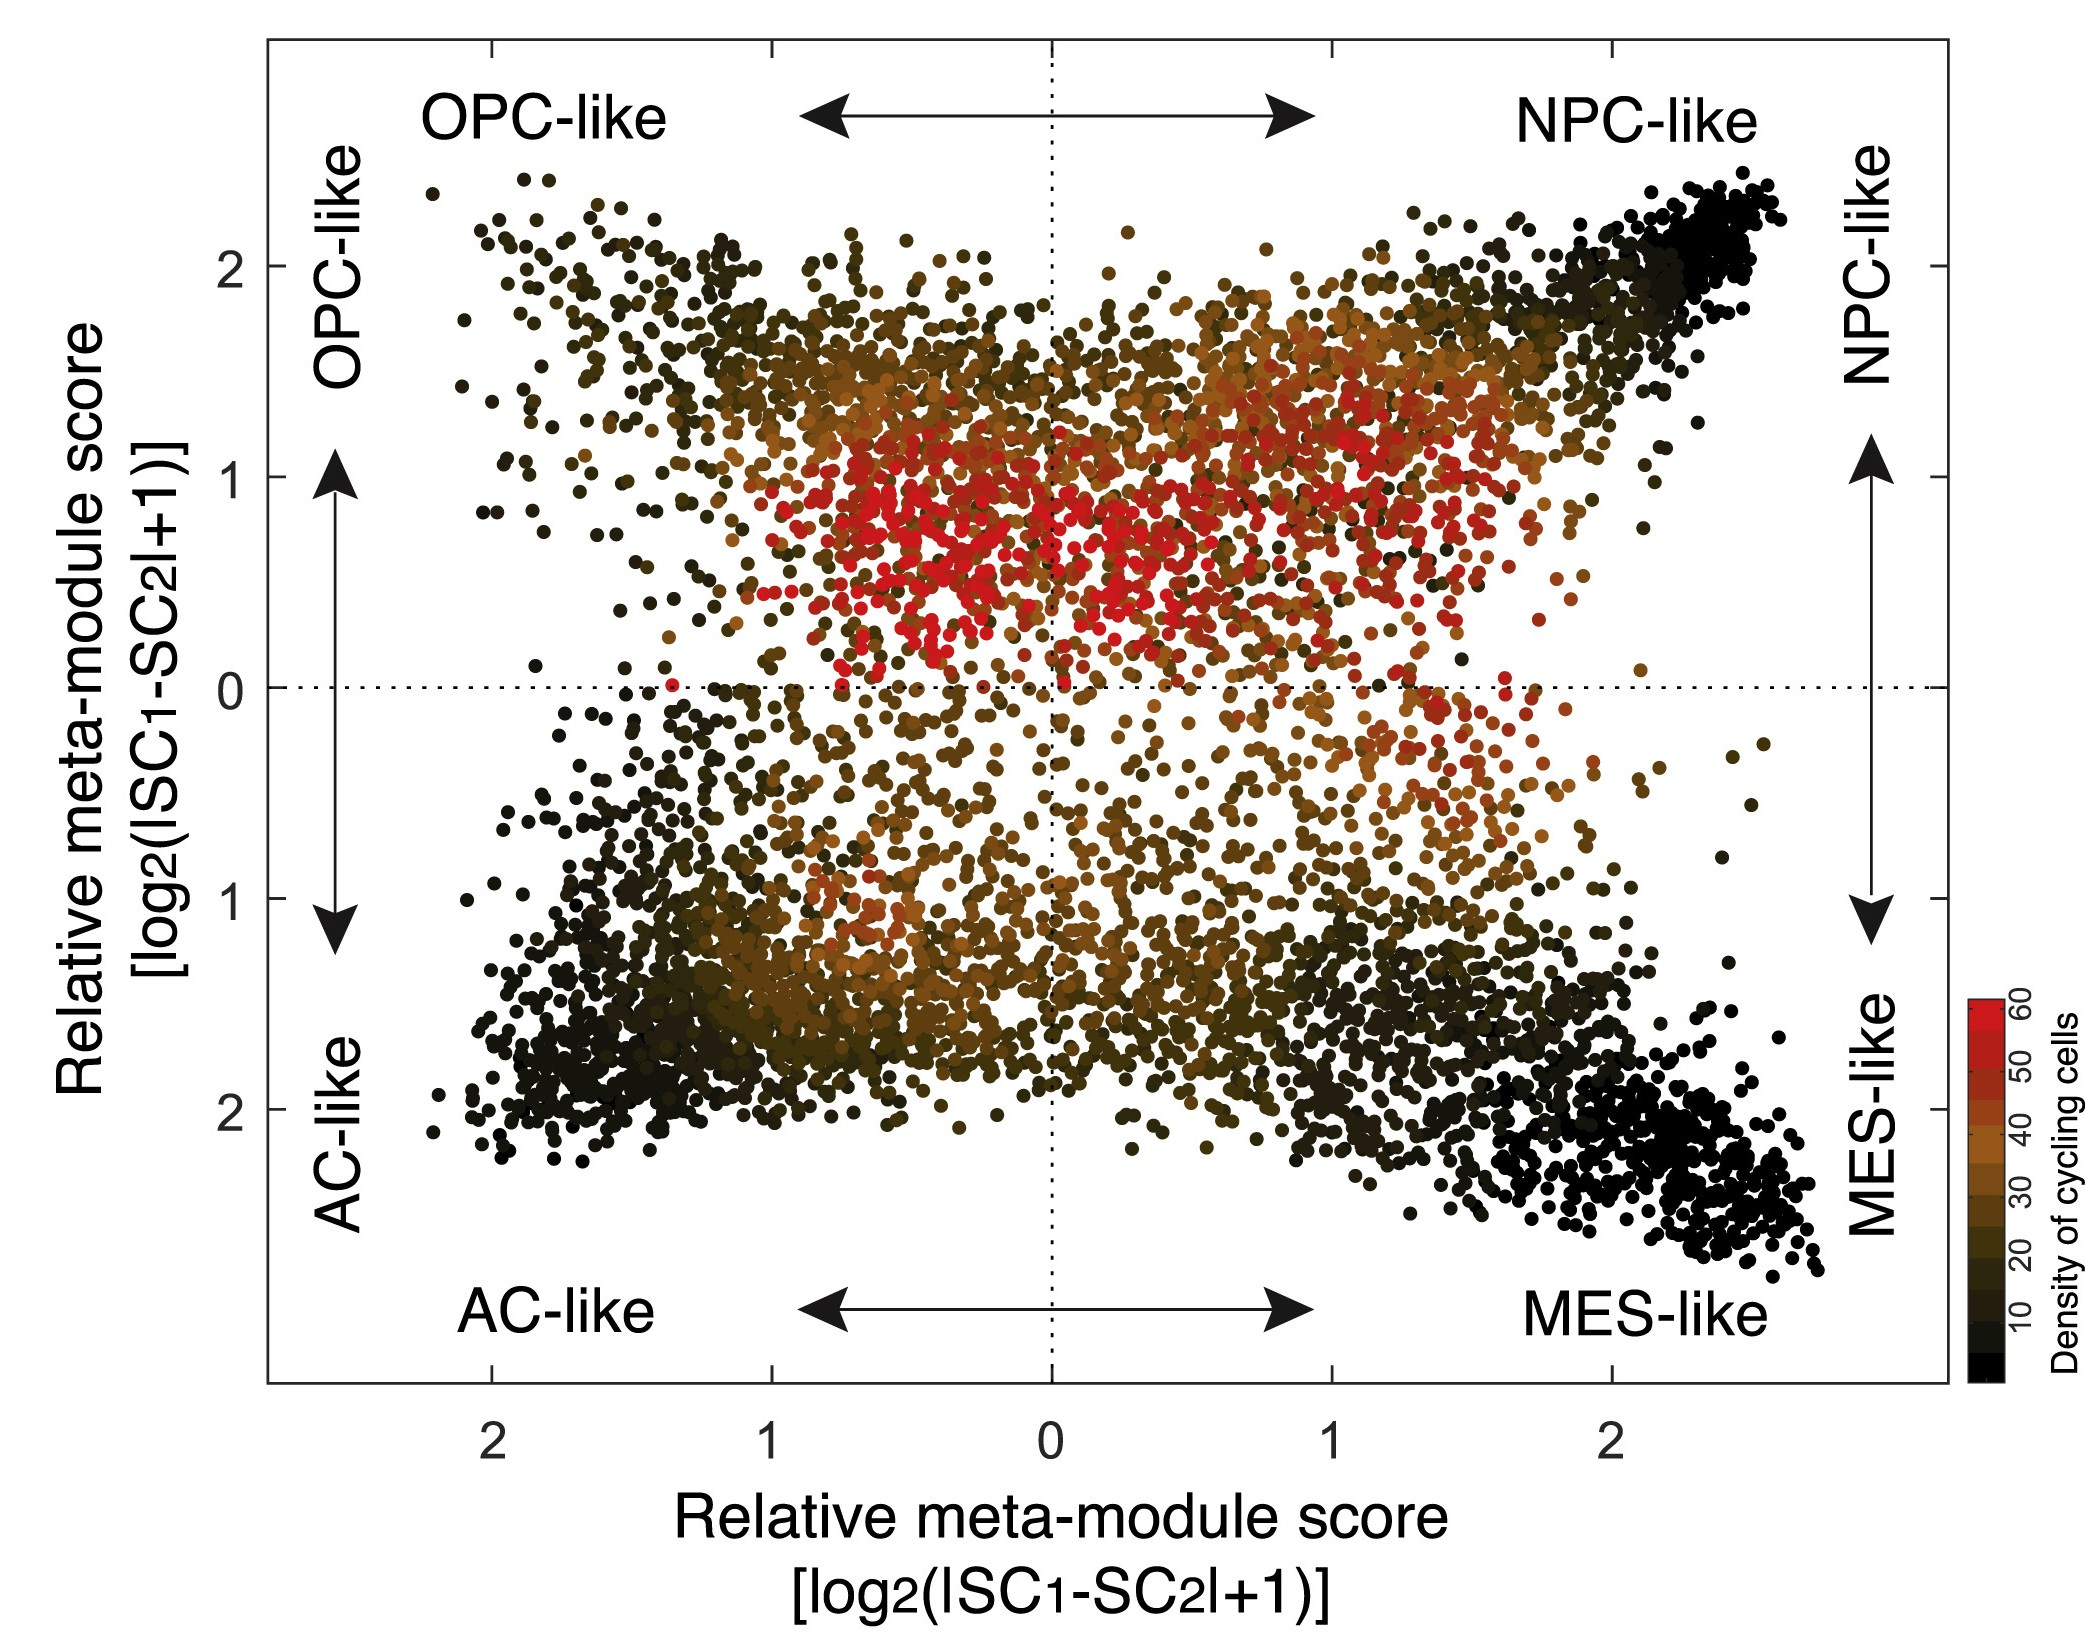
\includegraphics[width=\textwidth]{neftel_ninja_star}
                    \caption{Cell states by \cite{Neftel}}
                \end{subfigure}
                \pause[1]\caption{Cellular states defined for Glioblastoma (GBM)}
            \end{figure}
        \end{adjustwidth}
    \end{frame}

    \begin{frame}[standout]
        Are these cell states truly distinct and mutually exclusive?
    \end{frame}

%     \section{Preliminary results}

    \begin{frame}{Method for scoring signatures}
    \begin{columns}
    \begin{column}{0.55\textwidth}
        Scoring of Genesets: ssGSEA \footcite{ssGSEA}
        $$ES(G,S) = \sum_{i=1}^N \left[ \underbrace{\sum_{r\in G, j\le i}\frac{|r_j|^{(1/4)}}{\sum_{r_j\in G}|r_j|^{(1/4)}}}_{\text{ECDF of genes in signature}} - \underbrace{\sum_{r\notin G, j\le i} \frac{1}{N - N_G}}_{\text{ECDF of background genes}}\right]$$
        {\scriptsize Where,
        \begin{itemize}
            \item $G_i =$ Gene Set i
            \item $N_i =$ Number of genes in set i
            \item $r_j =$ Rank of gene j
            \item $\rho_r(x,y) =$ Spearman correlation of x scores with y scores
        \end{itemize}}
    \end{column}
    \begin{column}{0.45\textwidth}
        \begin{figure}
            \centering
            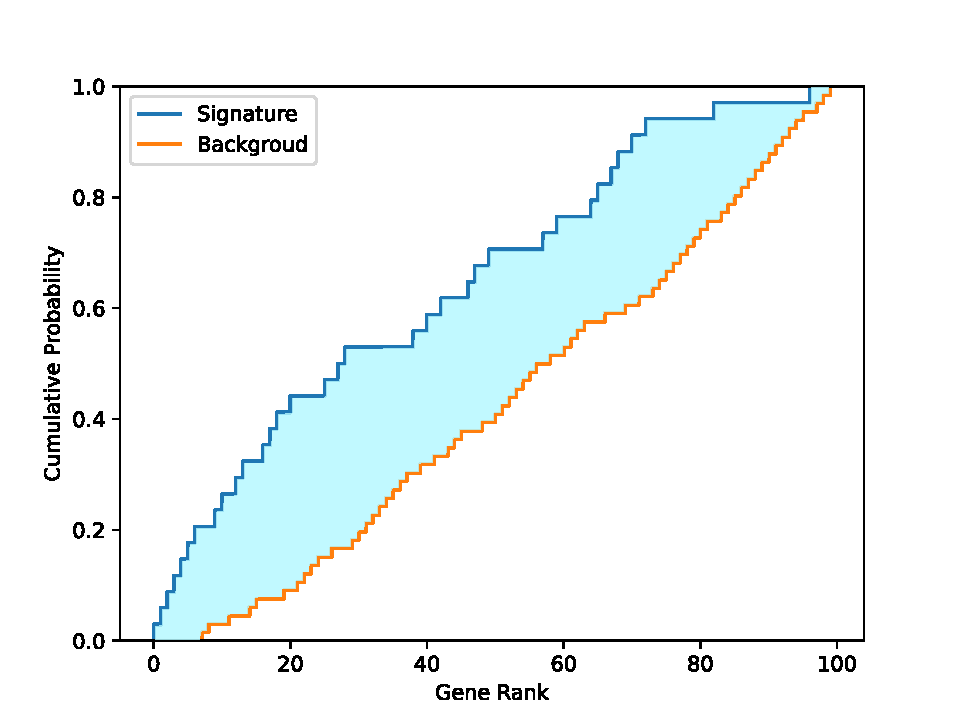
\includegraphics[width=\textwidth]{ecdf}
            \caption{Schematic of ssGSEA}
        \end{figure}
        \pause
        \begin{itemize}
            \item Antagonistic $\implies \rho_r(x,y) = -ve $
            \item Independent $\implies \rho_r(x,y) \approx 0 $
        \end{itemize}
    \end{column}
    \end{columns}
    \end{frame}
%     % Give explanation of why we expect -ve correlation

    \begin{frame}{Not all states are distinctly mutually antagonistic (Neftel)}
        \begin{adjustwidth}{-5cm}{-5cm}
            \centering
            \begin{figure}
                \centering
                \begin{subfigure}[c]{0.4\textwidth}
                    \centering
                    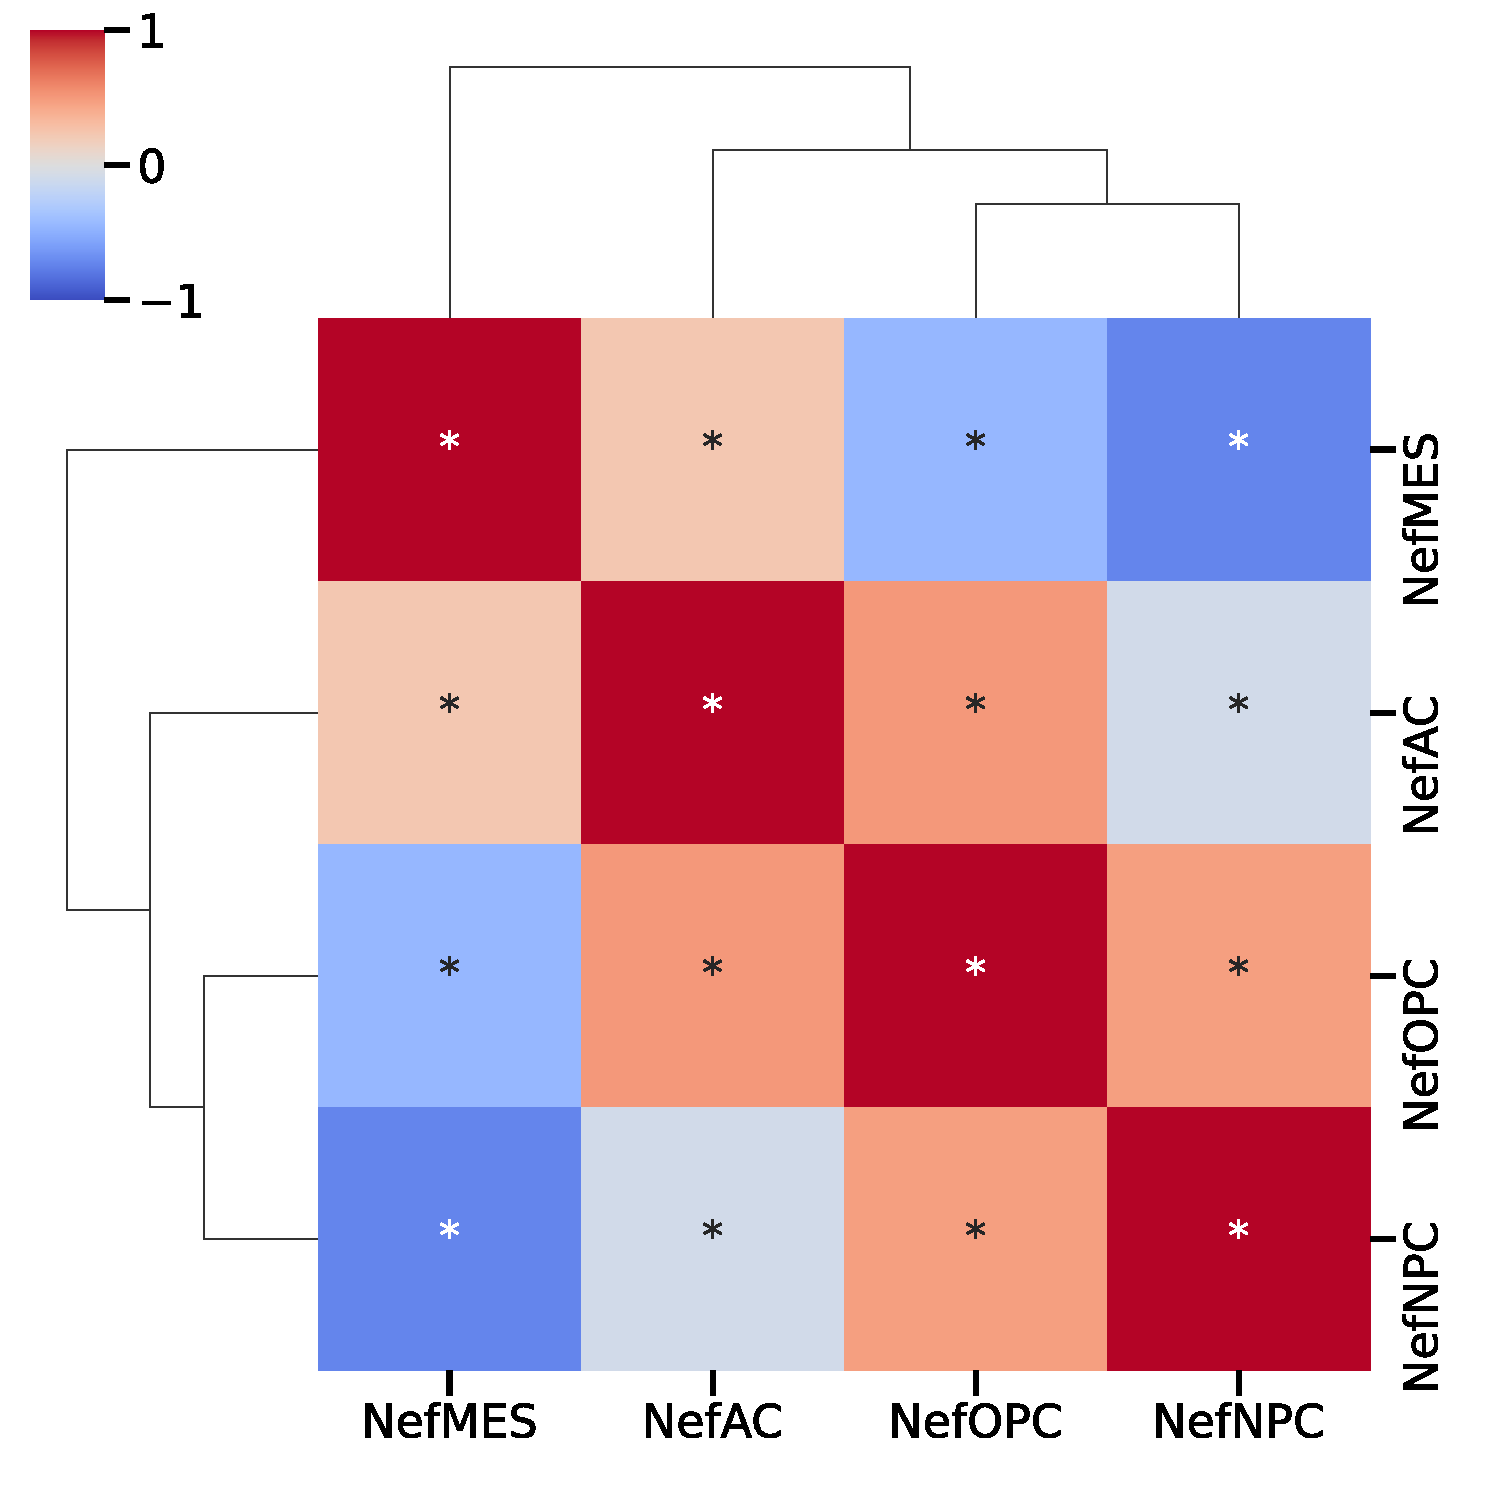
\includegraphics[width=\textwidth]{GSEA_GSM3828672_corrplot_Nef}
                    \caption{GSE131928}
                \end{subfigure}
                \begin{subfigure}[c]{0.4\textwidth}
                    \centering
                    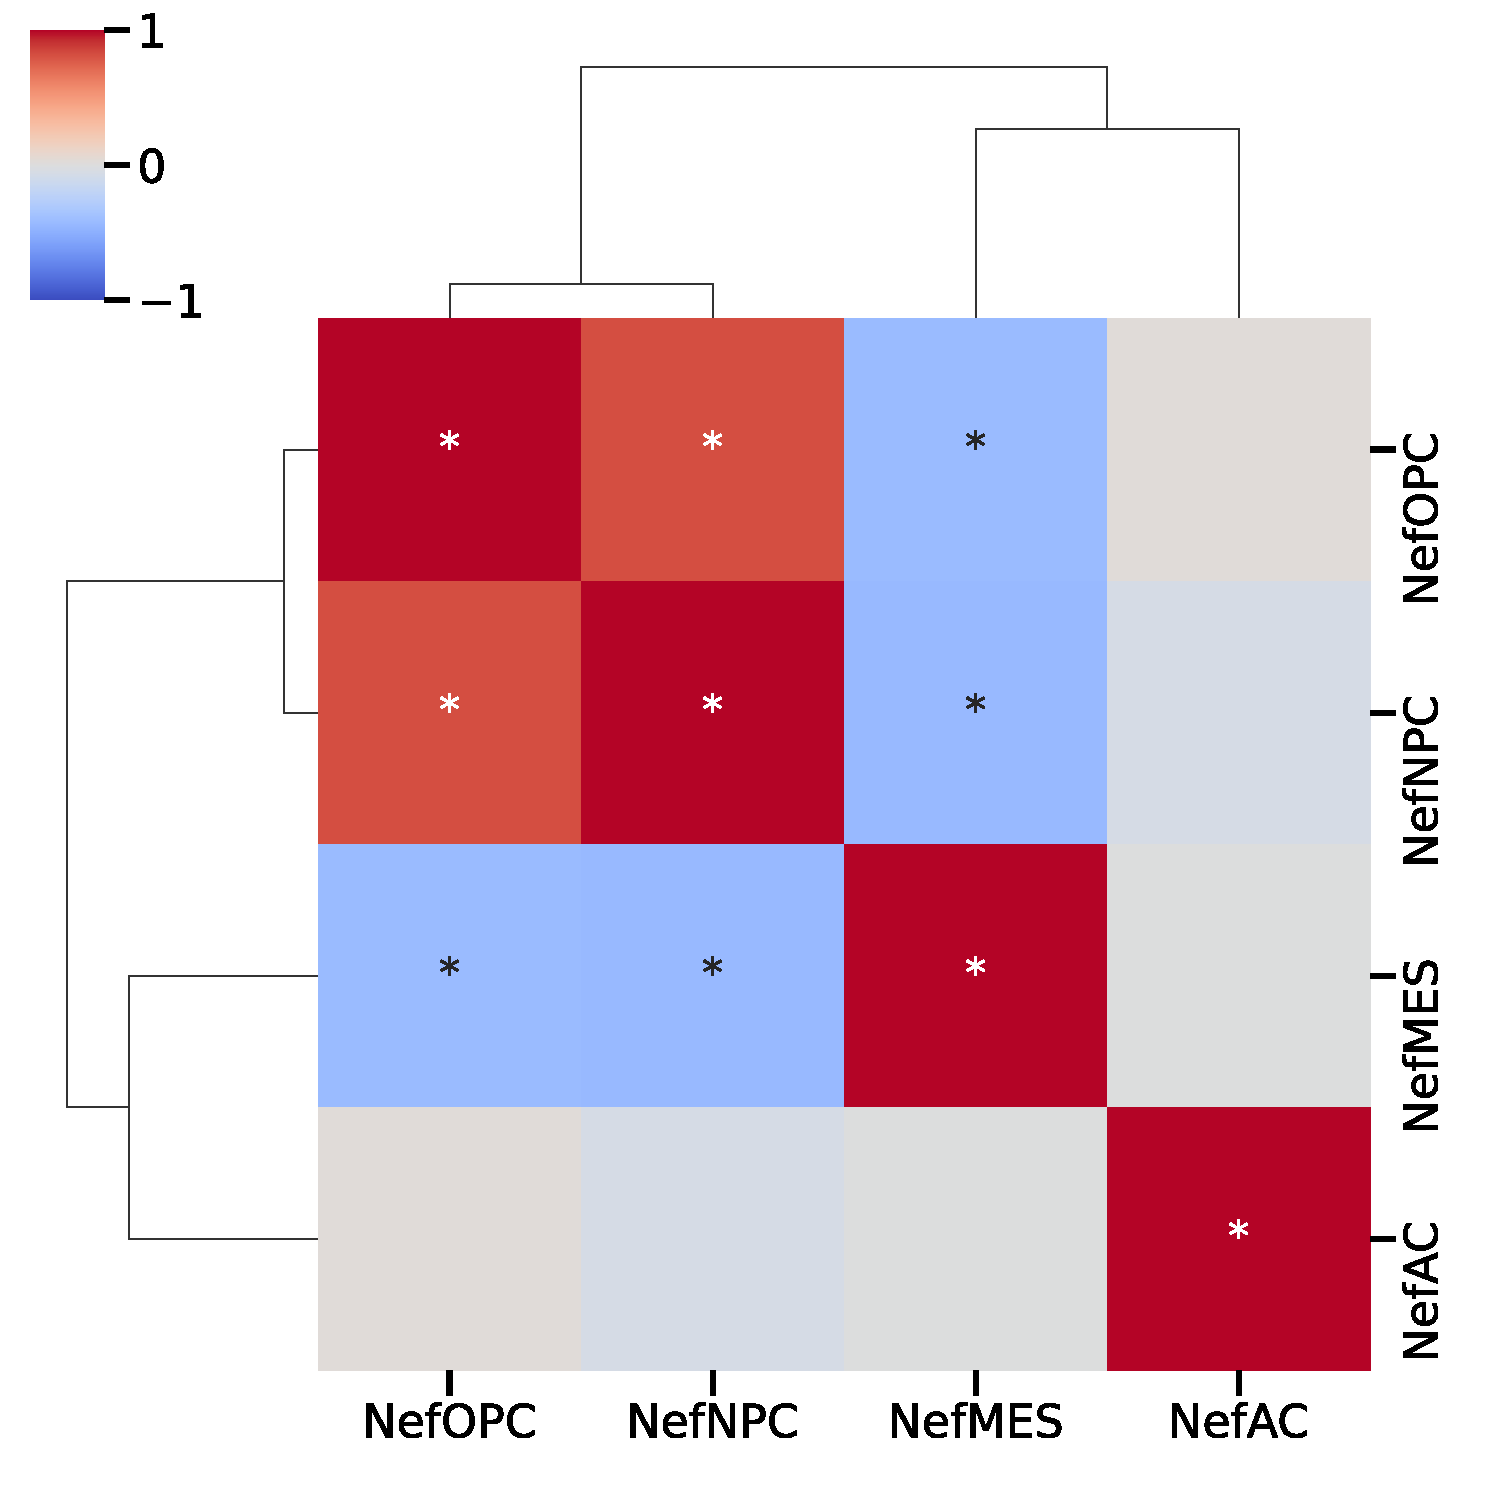
\includegraphics[width=\textwidth]{GSEA_TCGA_corrplot_Nef}
                    \caption{TCGA}
                \end{subfigure}
                \caption{Correlation of ssGSEA/AUCell scores}
            \end{figure}
        \end{adjustwidth}
    \end{frame}

    \begin{frame}{Not all states are distinctly mutually antagonistic (Verhaak)}
        \begin{adjustwidth}{-5cm}{-5cm}
            \centering
            \begin{figure}\ContinuedFloat
                \centering
                \begin{subfigure}[c]{0.4\textwidth}
                    \centering
                    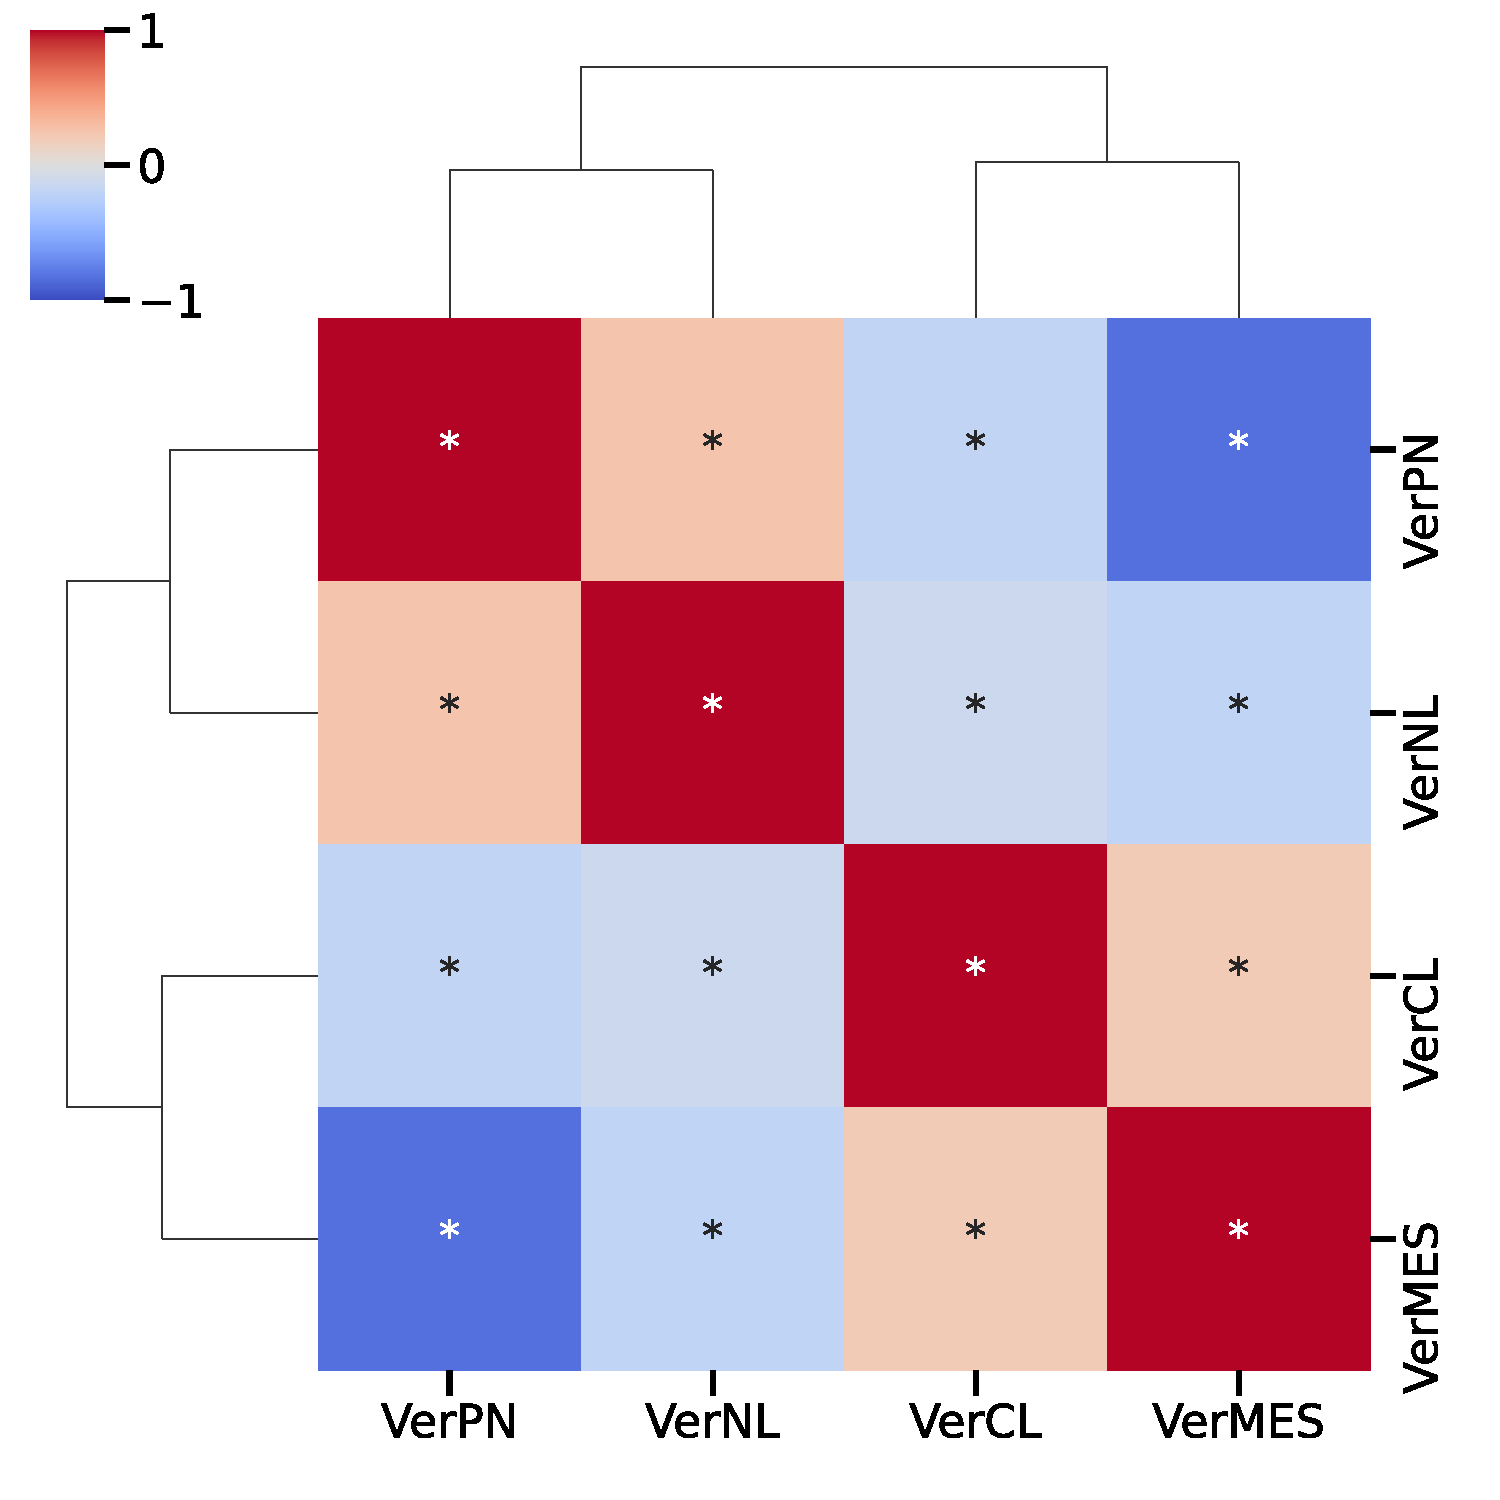
\includegraphics[width=\textwidth]{GSEA_GSM3828672_corrplot_Ver}
                    \caption{GSE131928}
                \end{subfigure}
                \begin{subfigure}[c]{0.4\textwidth}
                    \centering
                    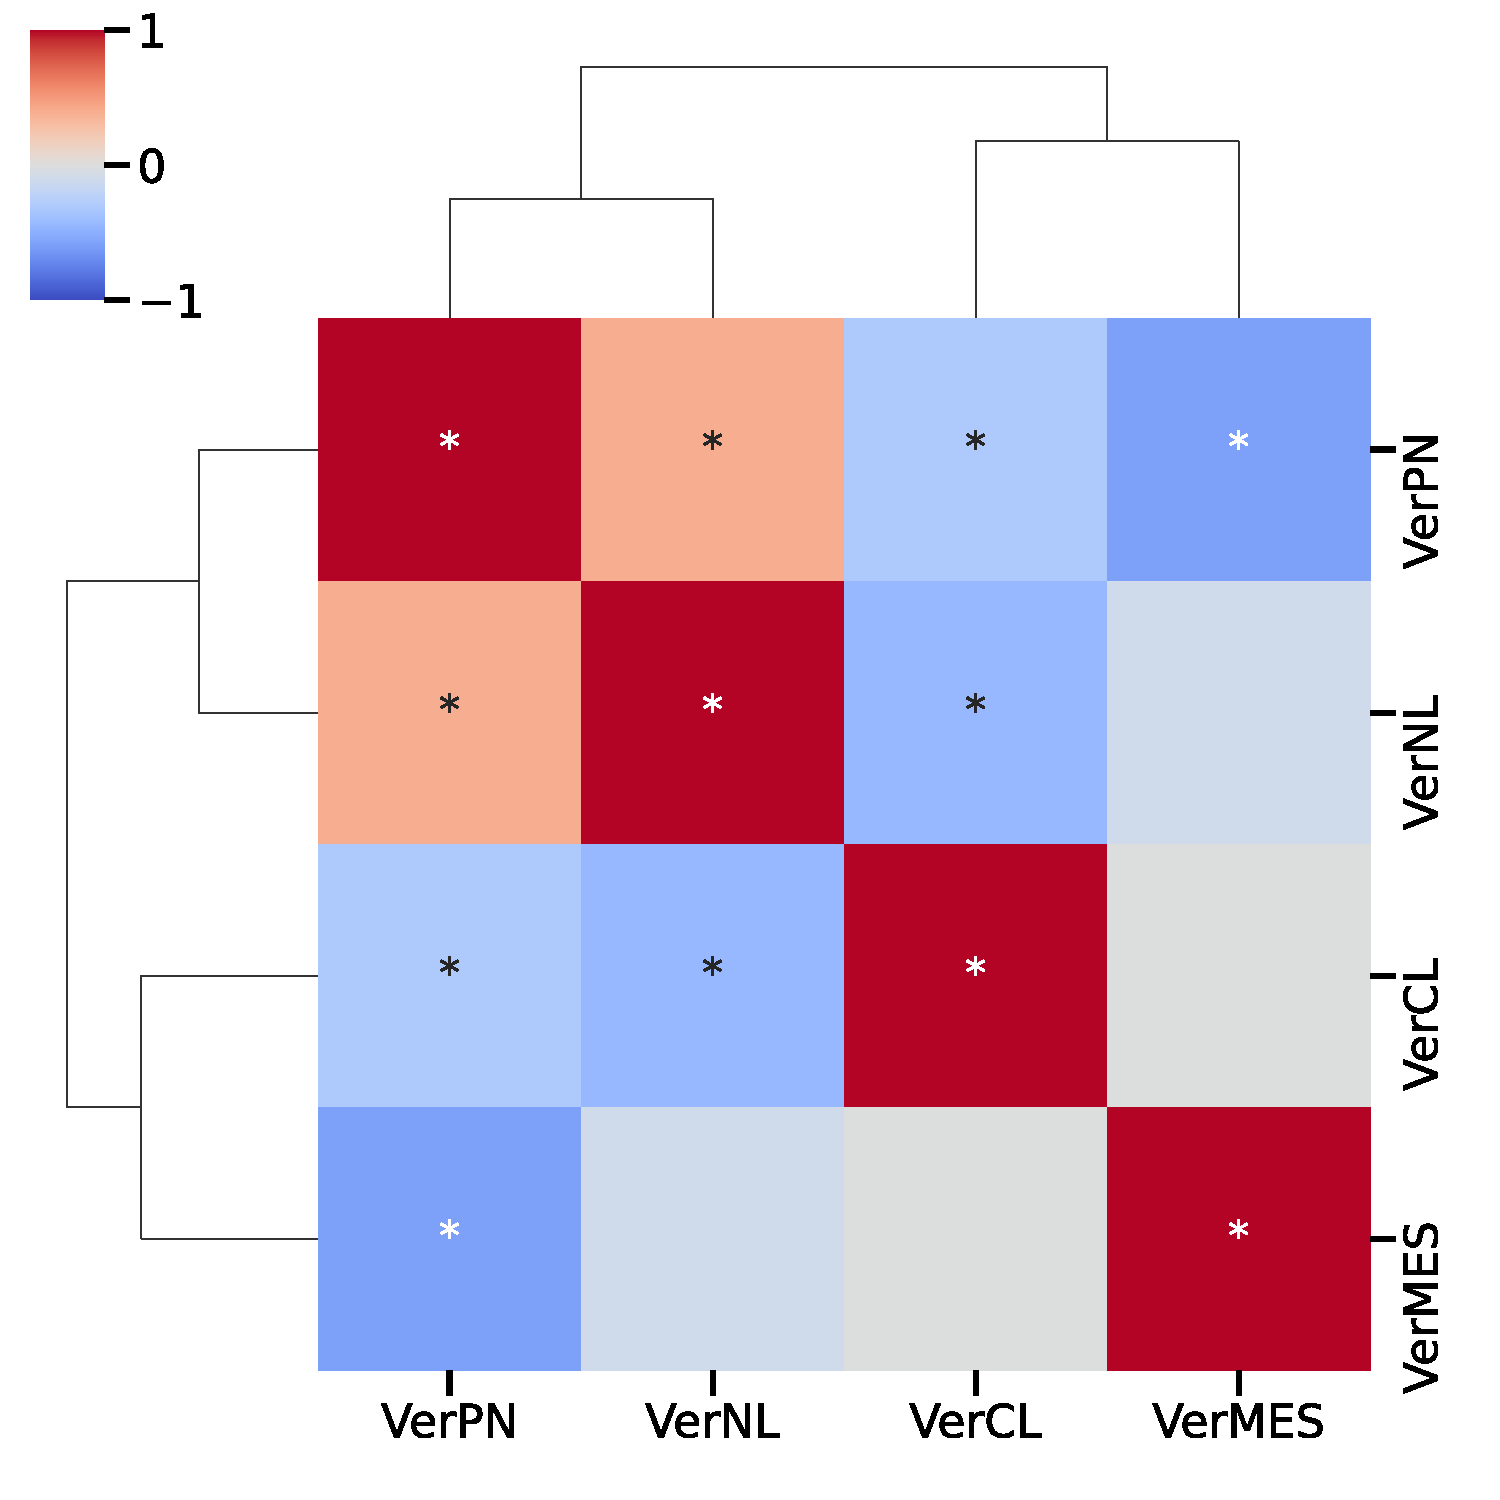
\includegraphics[width=\textwidth]{GSEA_TCGA_corrplot_Ver}
                    \caption{TCGA}
                \end{subfigure}
                \caption{Correlation of ssGSEA/AUCell scores}
            \end{figure}
        \end{adjustwidth}
    \end{frame}

    \begin{frame}{Similar states between Neftel and Verhaak}
        \begin{adjustwidth}{-5cm}{-5cm}
            \centering
            \begin{figure}\ContinuedFloat
                \centering
                \begin{subfigure}[c]{0.4\textwidth}
                    \centering
                    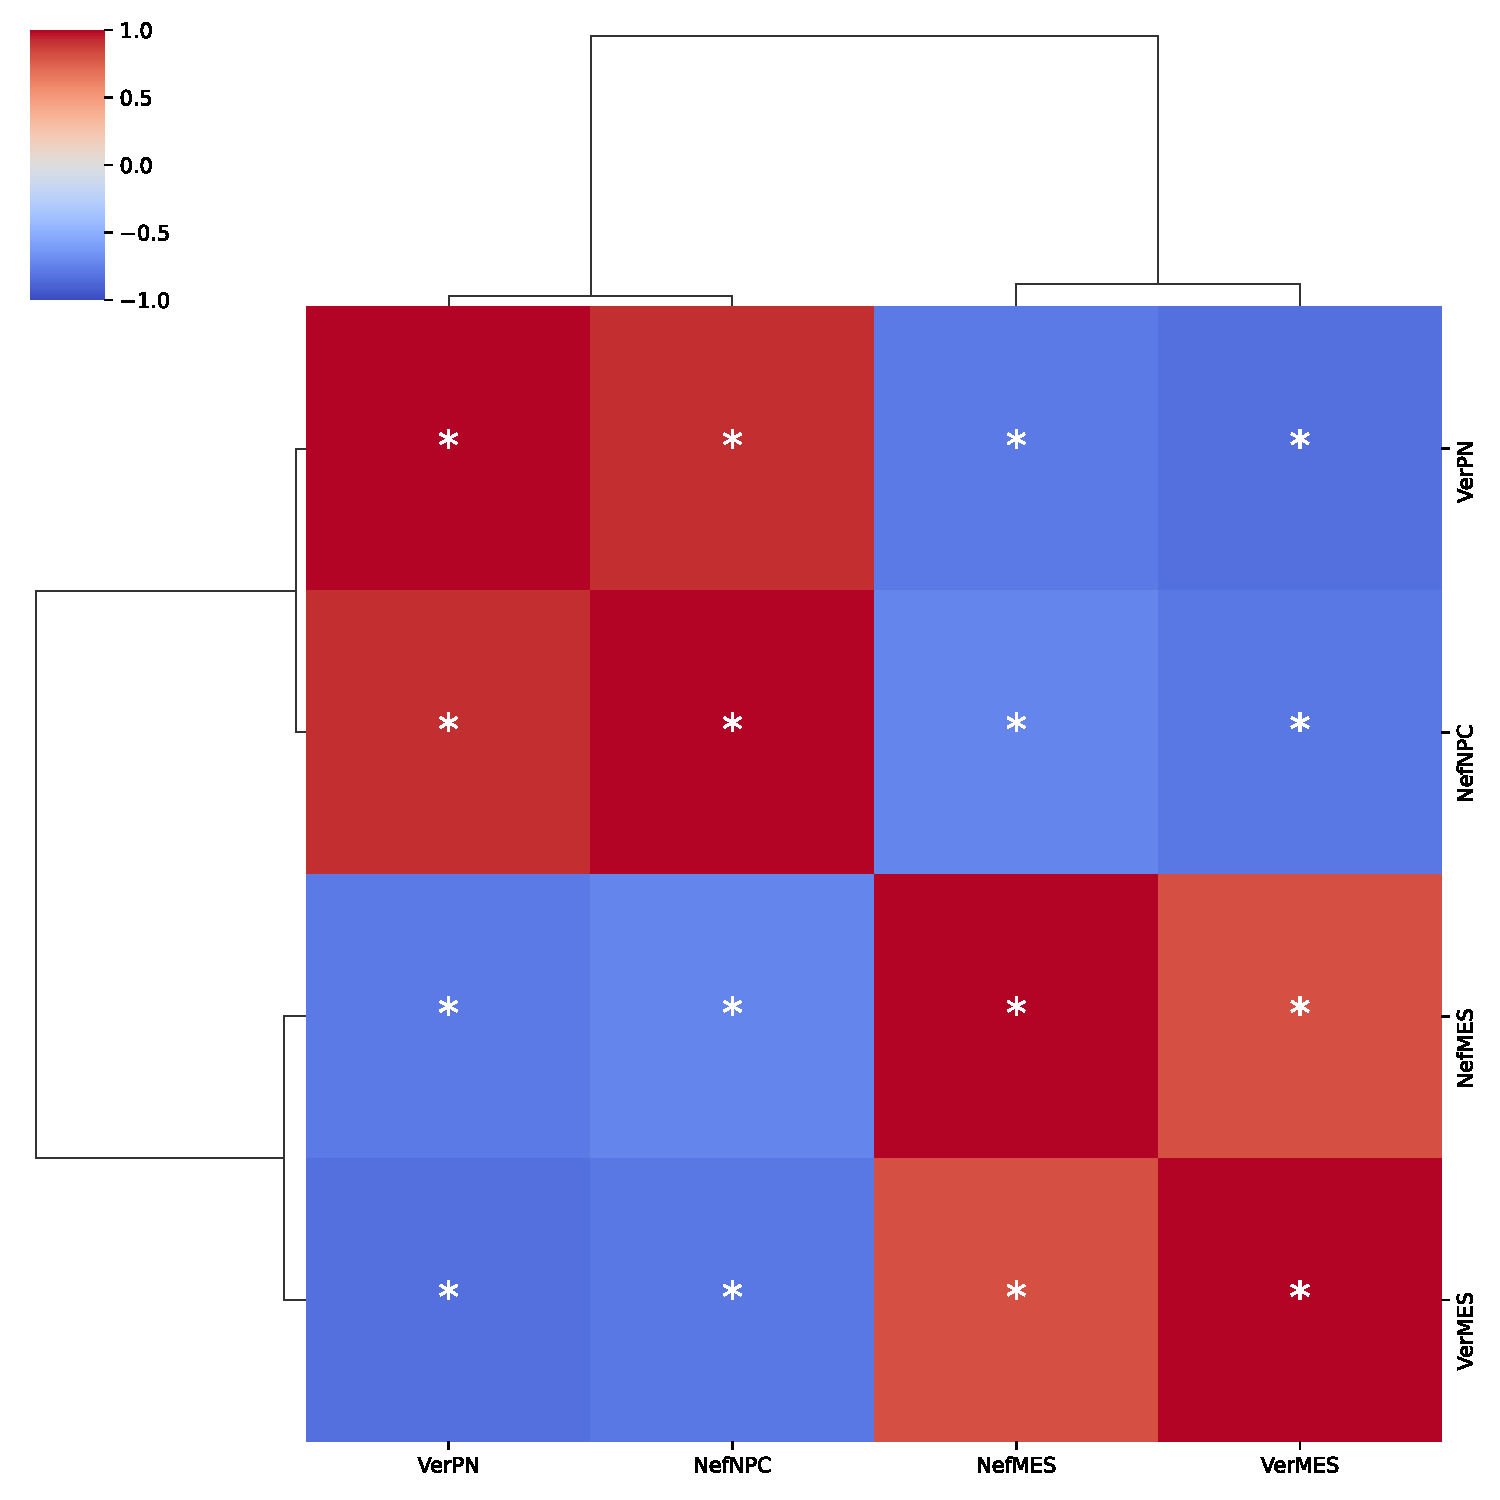
\includegraphics[width=\textwidth]{GSEA_GSM3828672_corrplot_2D}
                    \caption{GSE131928}
                \end{subfigure}
                \begin{subfigure}[c]{0.4\textwidth}
                    \centering
                    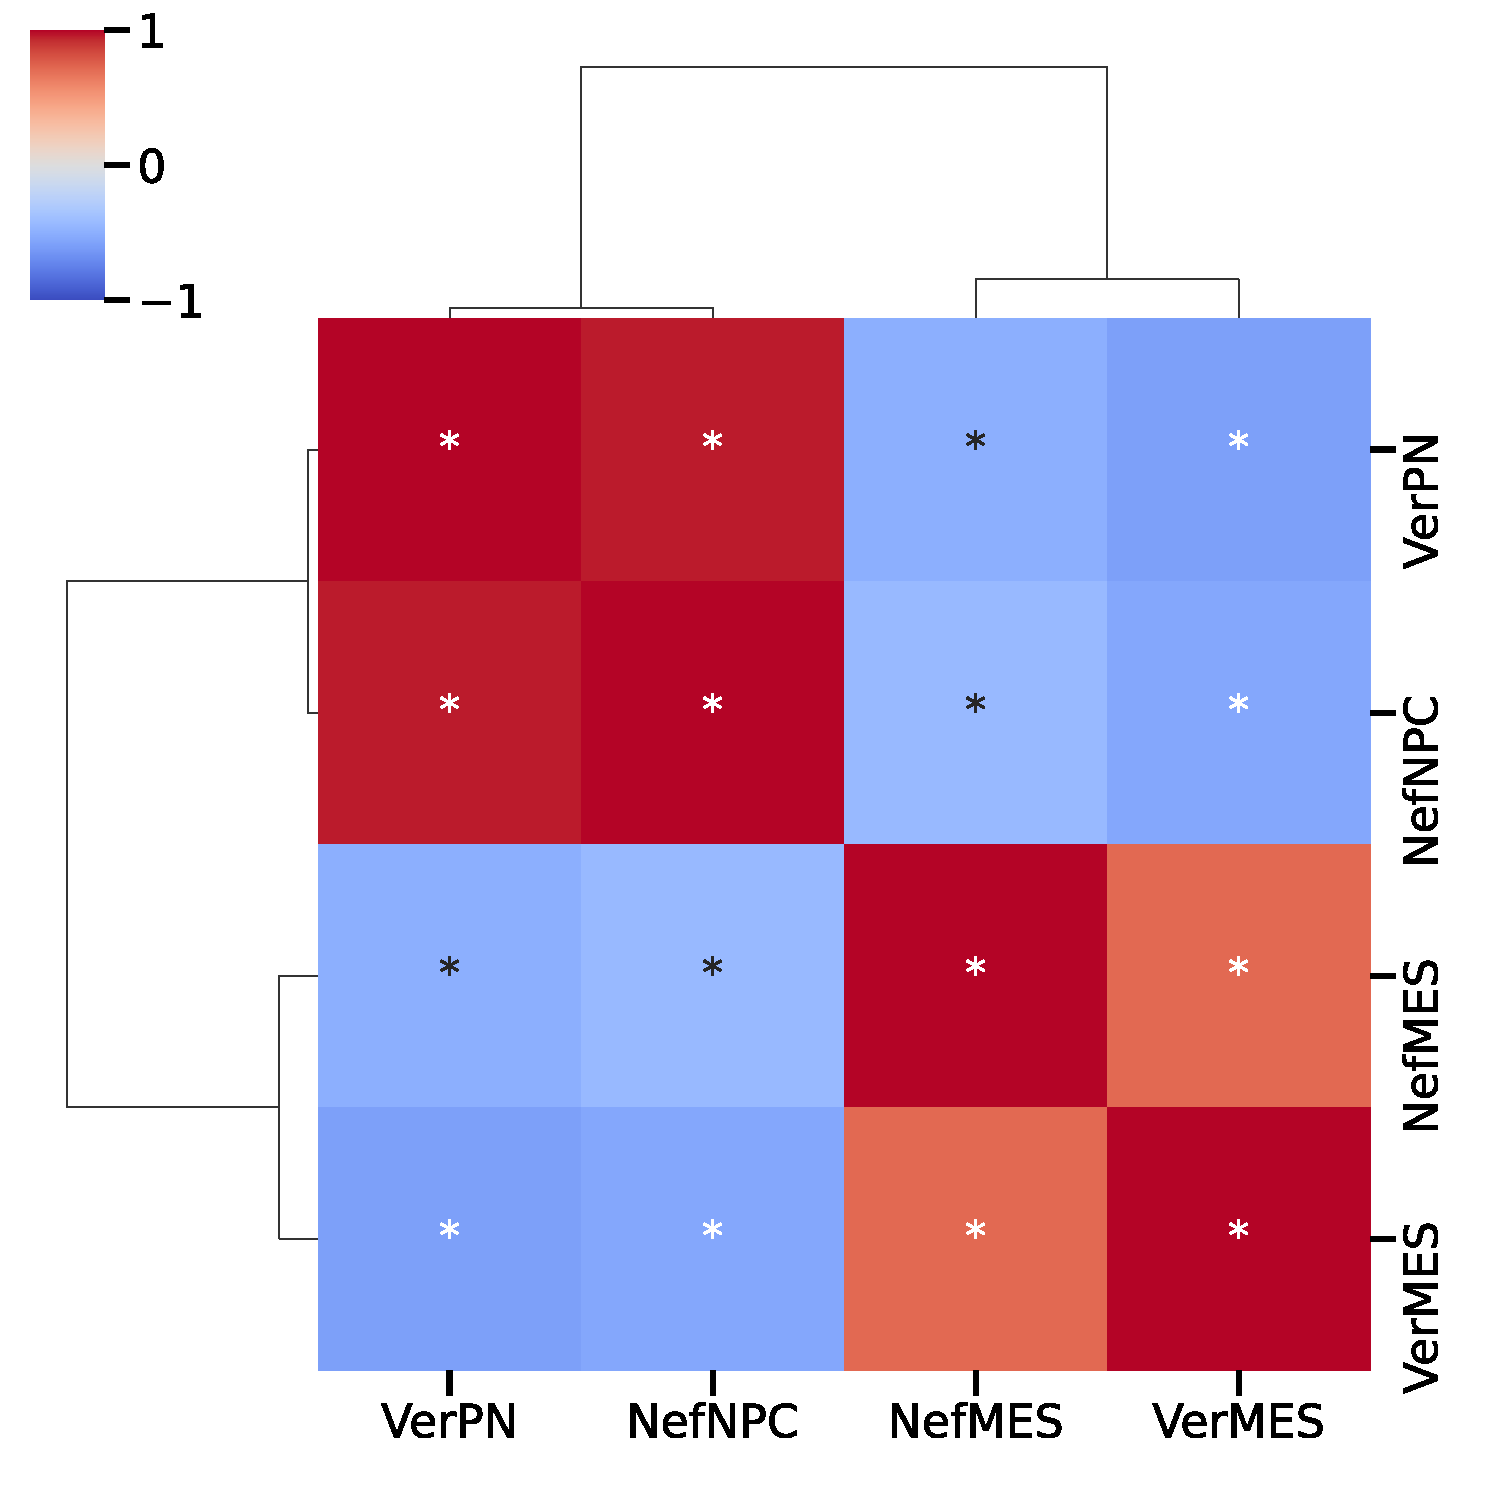
\includegraphics[width=\textwidth]{GSEA_TCGA_corrplot_2D}
                    \caption{TCGA}
                \end{subfigure}
                \caption{Correlation of ssGSEA/AUCell scores}
            \end{figure}
        \end{adjustwidth}
    \end{frame}

    \begin{frame}{Correlation of Expression also captures the NPC-MES antagonism (Neftel)}
        \begin{adjustwidth}{-5cm}{-5cm}
            \centering
            \begin{figure}
                \centering
                \begin{subfigure}[c]{0.48\textwidth}
                    \centering
                    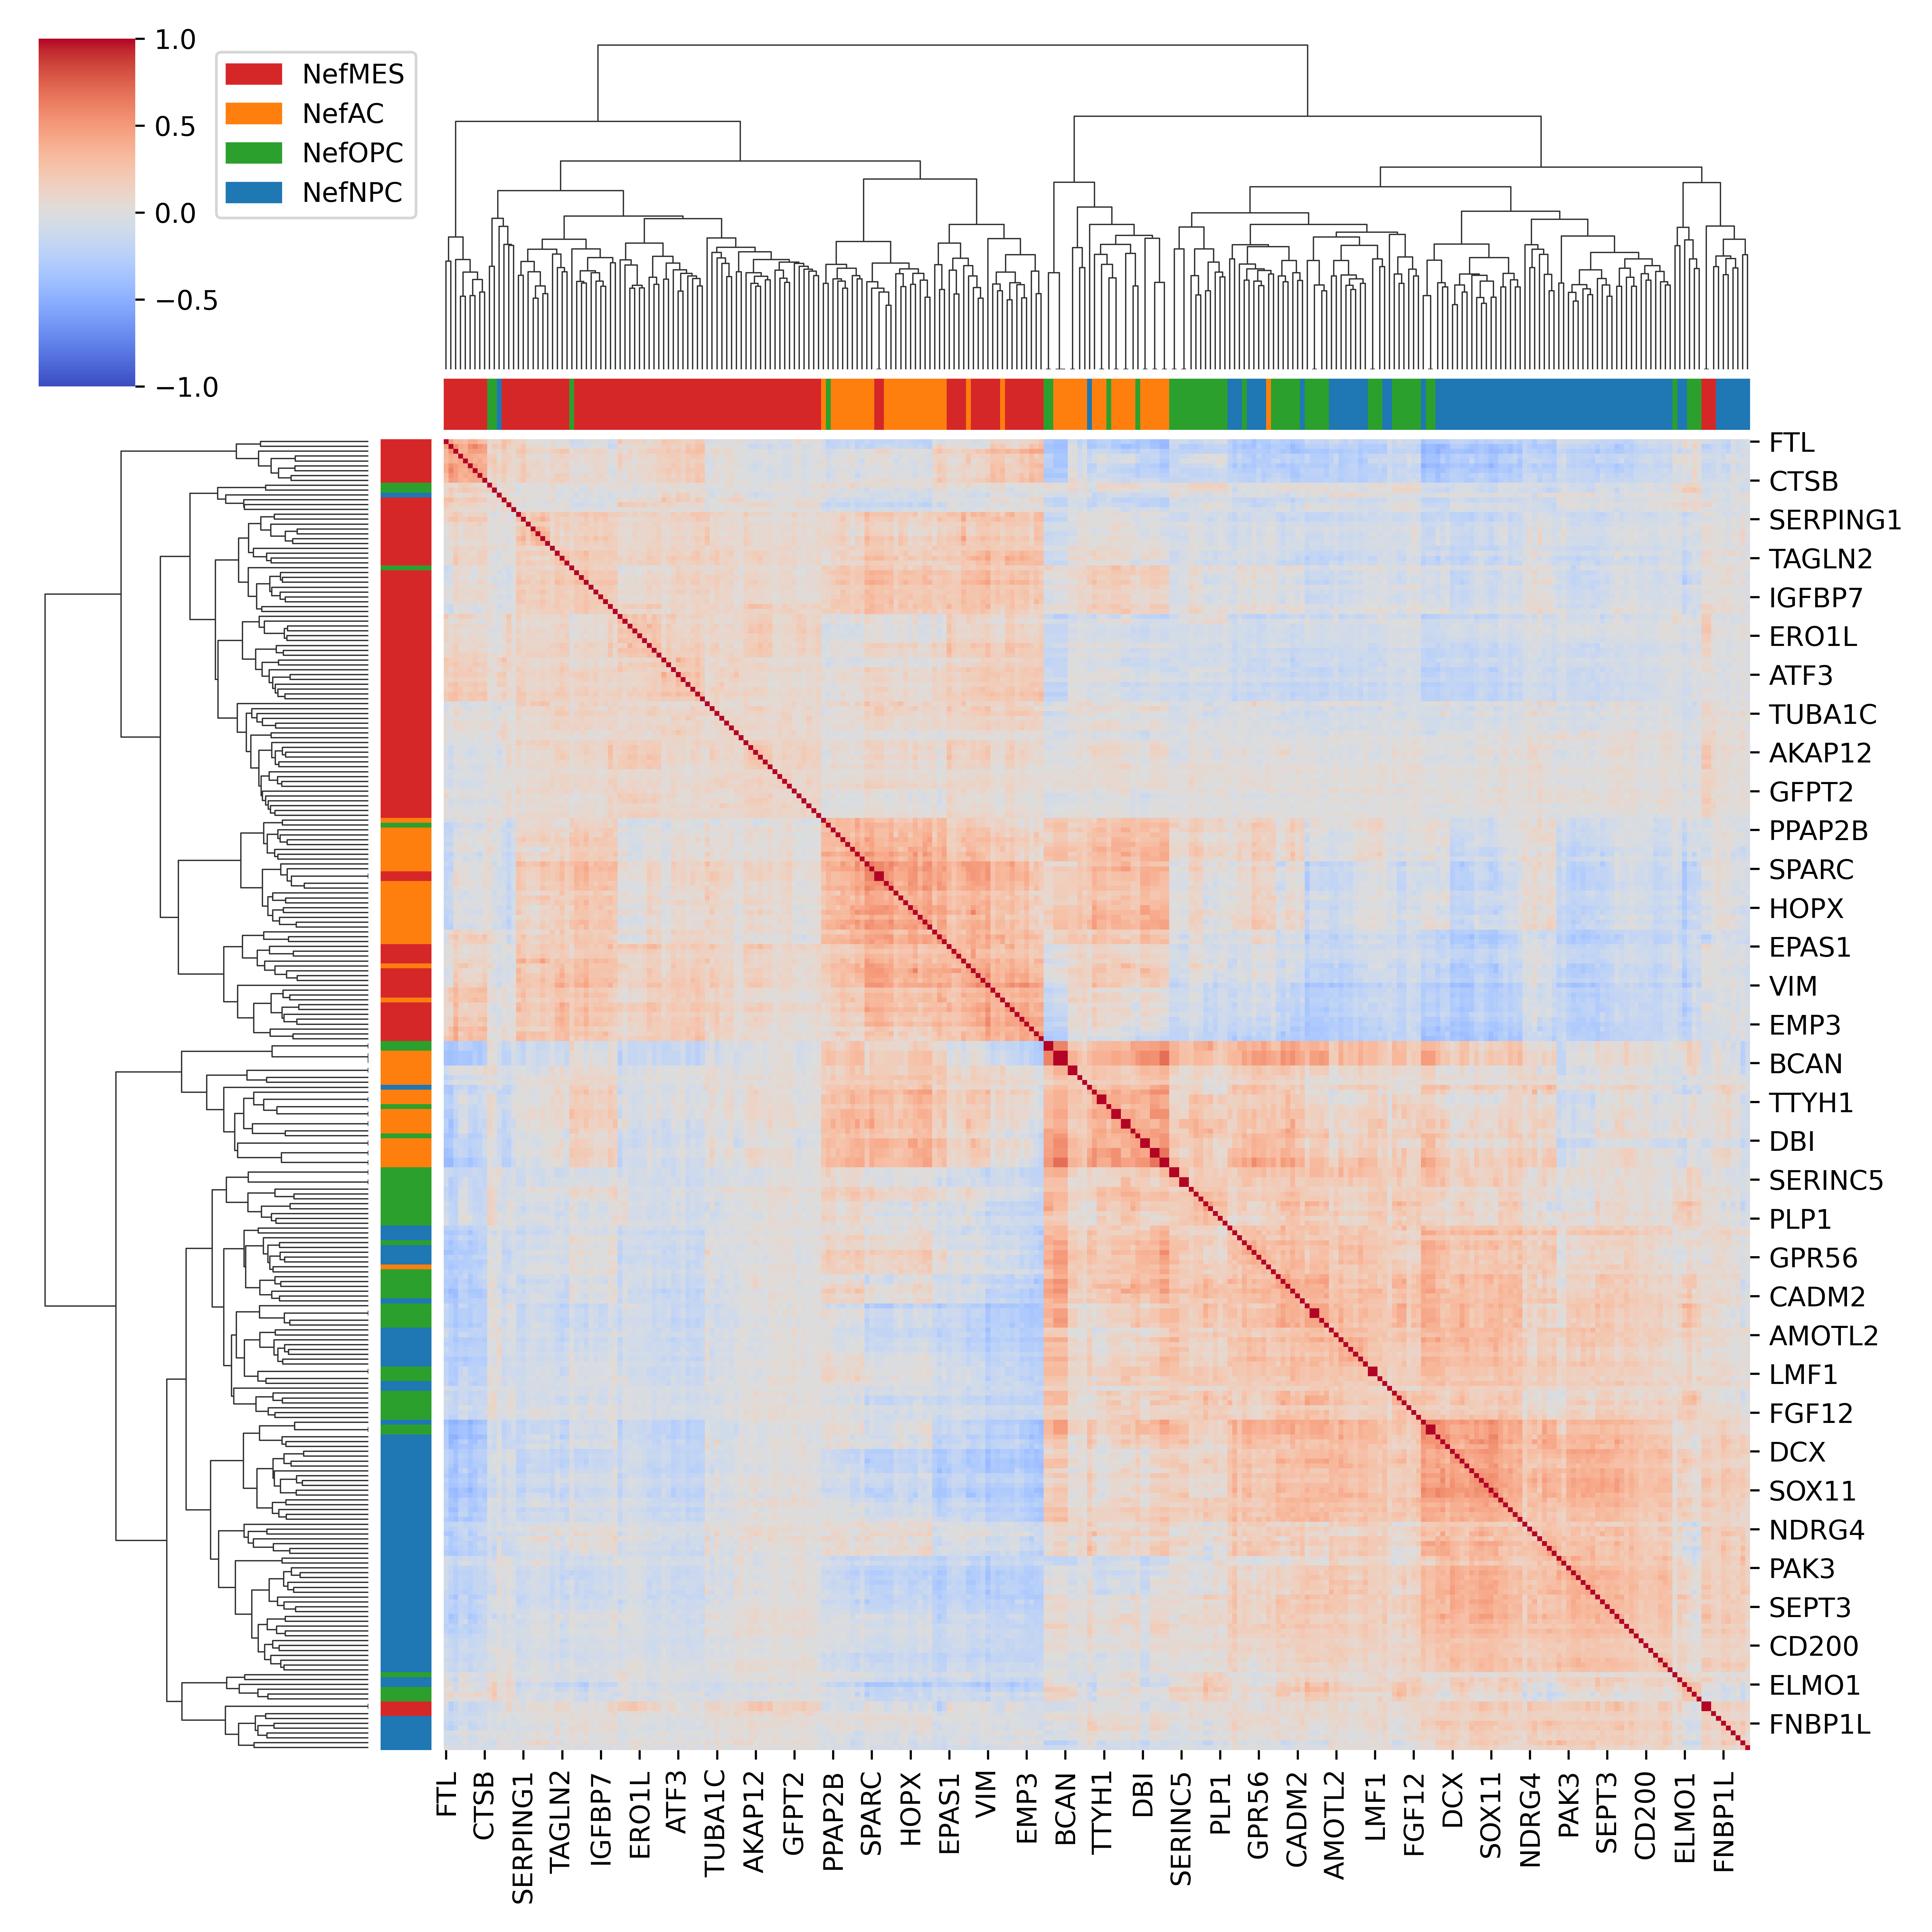
\includegraphics[width=\textwidth]{GSM3828672_Corrplot_Nef}
                    \caption{GSE131928}
                \end{subfigure}
                \begin{subfigure}[c]{0.48\textwidth}
                    \centering
                    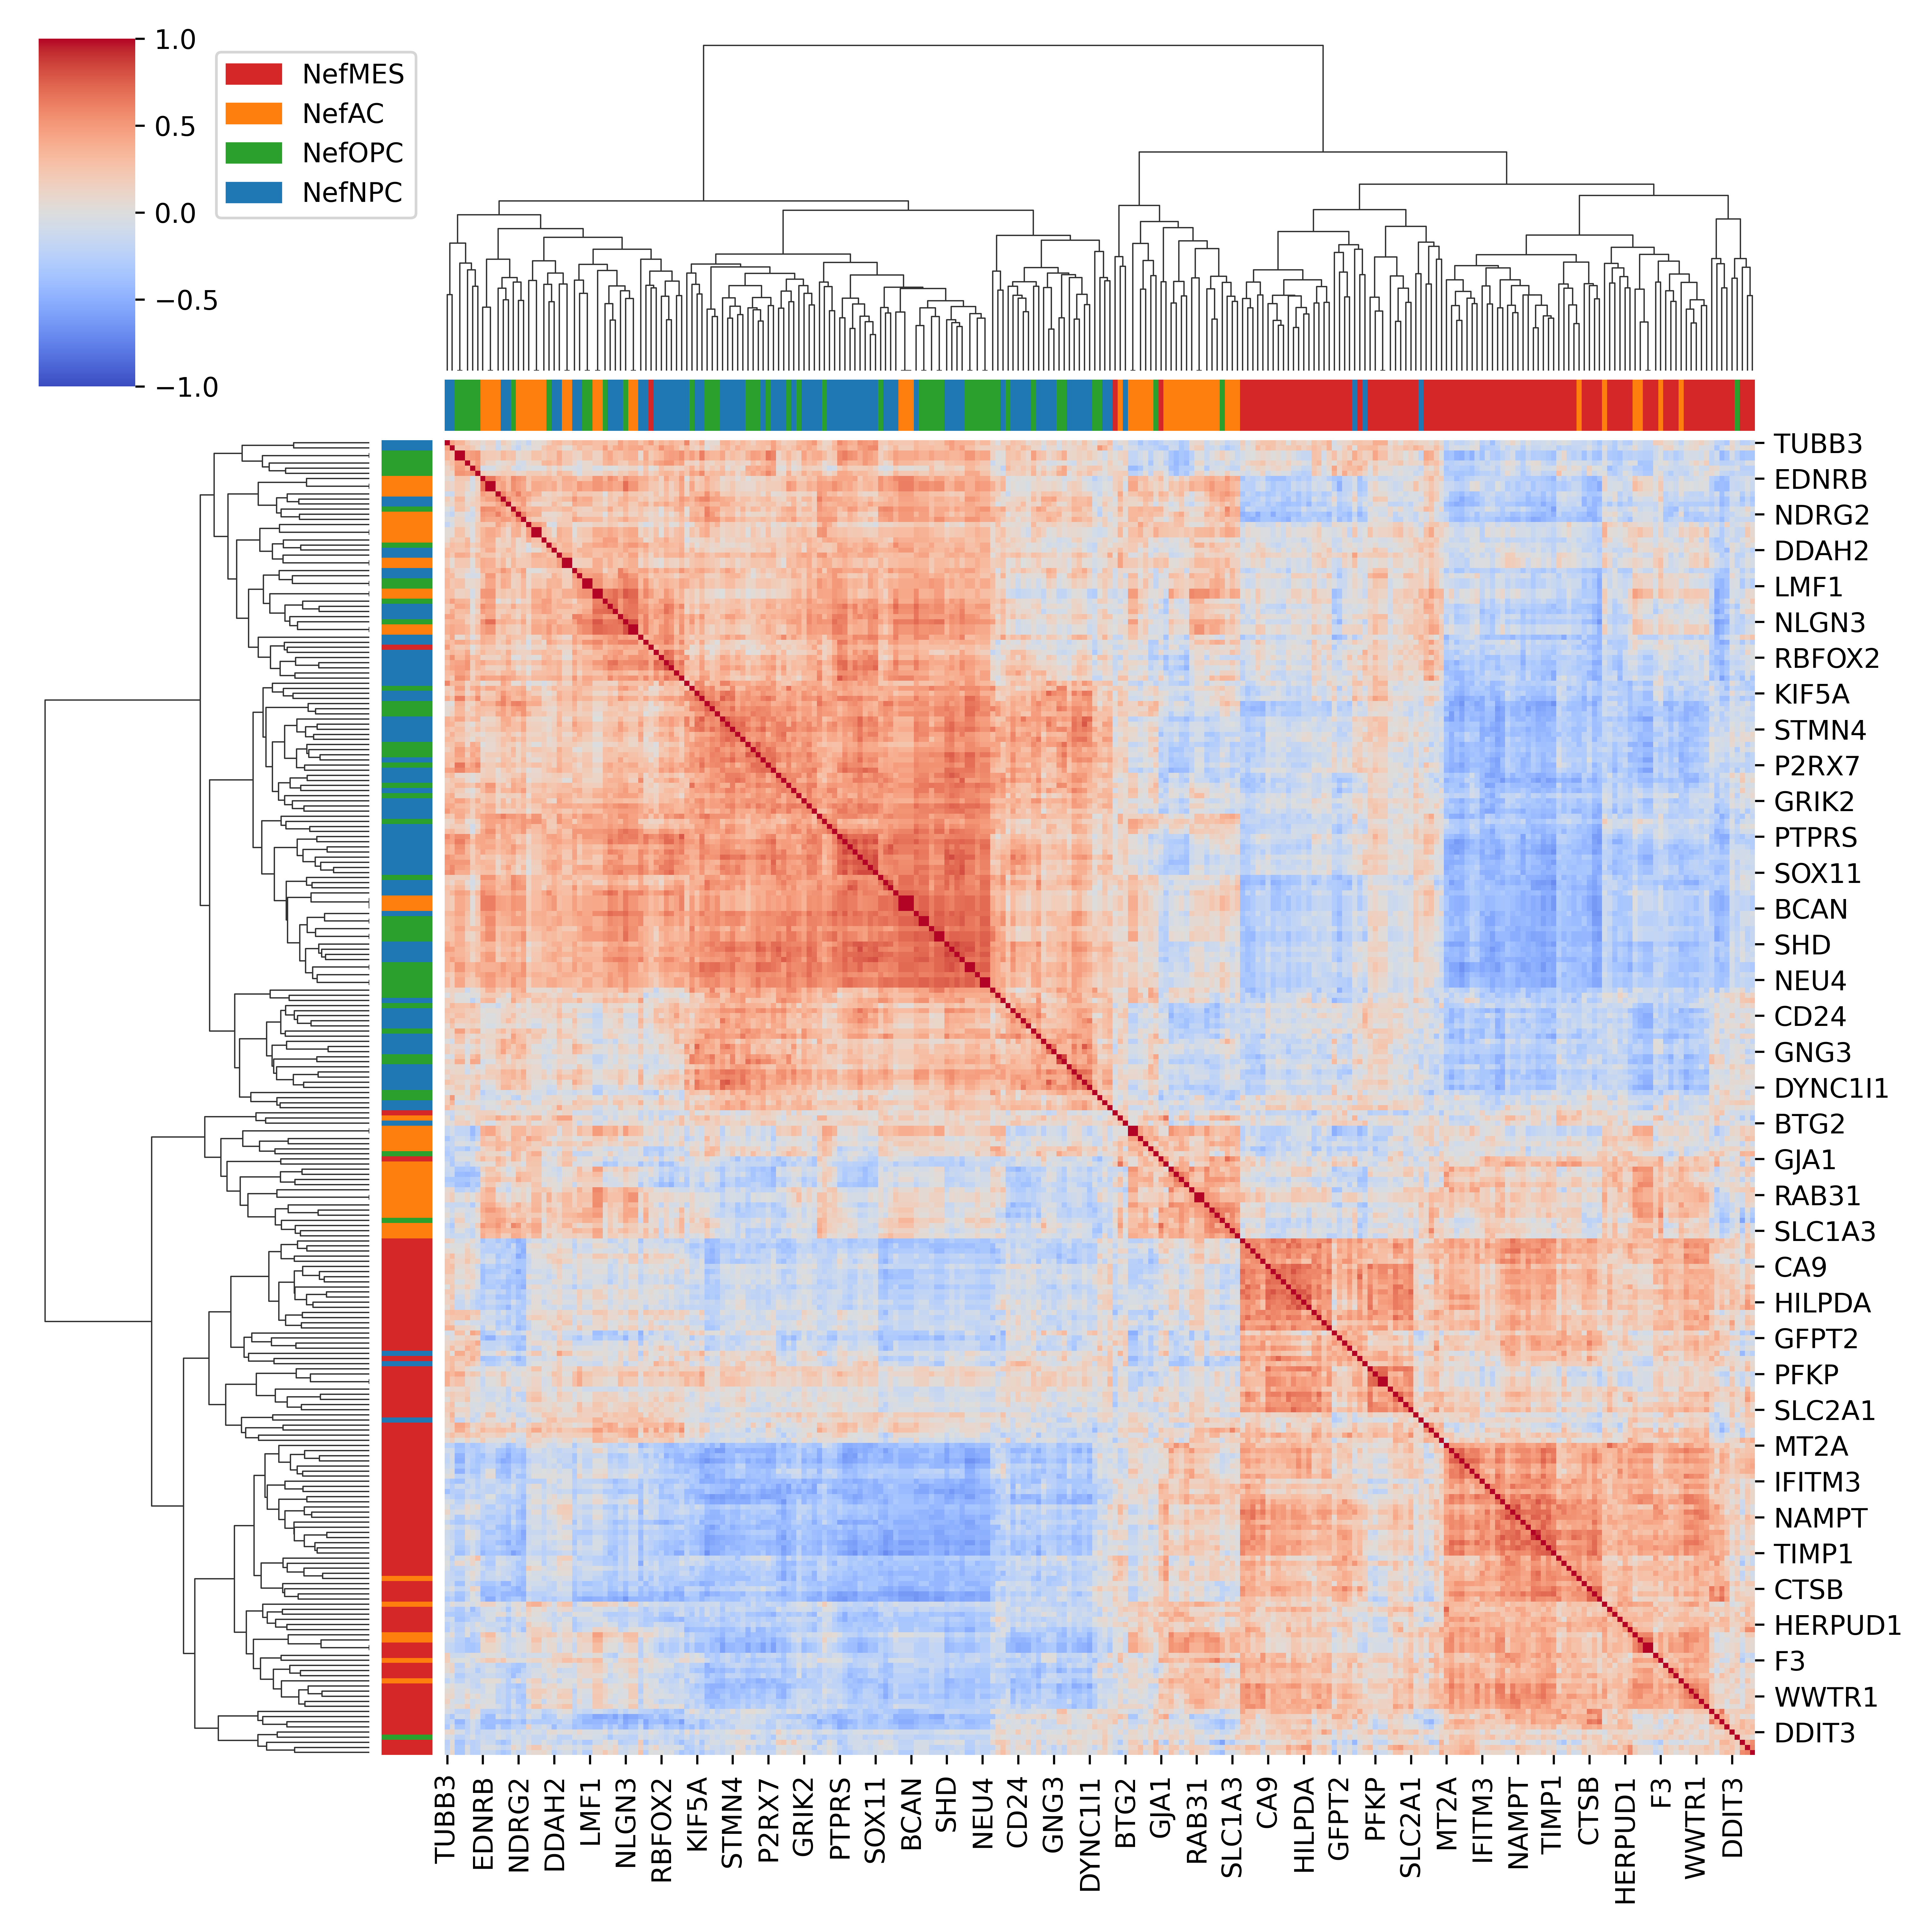
\includegraphics[width=\textwidth]{TCGA_Corrplot_Nef}
                    \caption{TCGA}
                \end{subfigure}
                \caption{Correlation of signature expression}
            \end{figure}
        \end{adjustwidth}
    \end{frame}

    \begin{frame}{Correlation of Expression also captures the PN-MES antagonism (Verhaak)}
        \begin{adjustwidth}{-5cm}{-5cm}
            \centering
            \begin{figure}\ContinuedFloat
                \centering
                \begin{subfigure}[c]{0.48\textwidth}
                    \centering
                    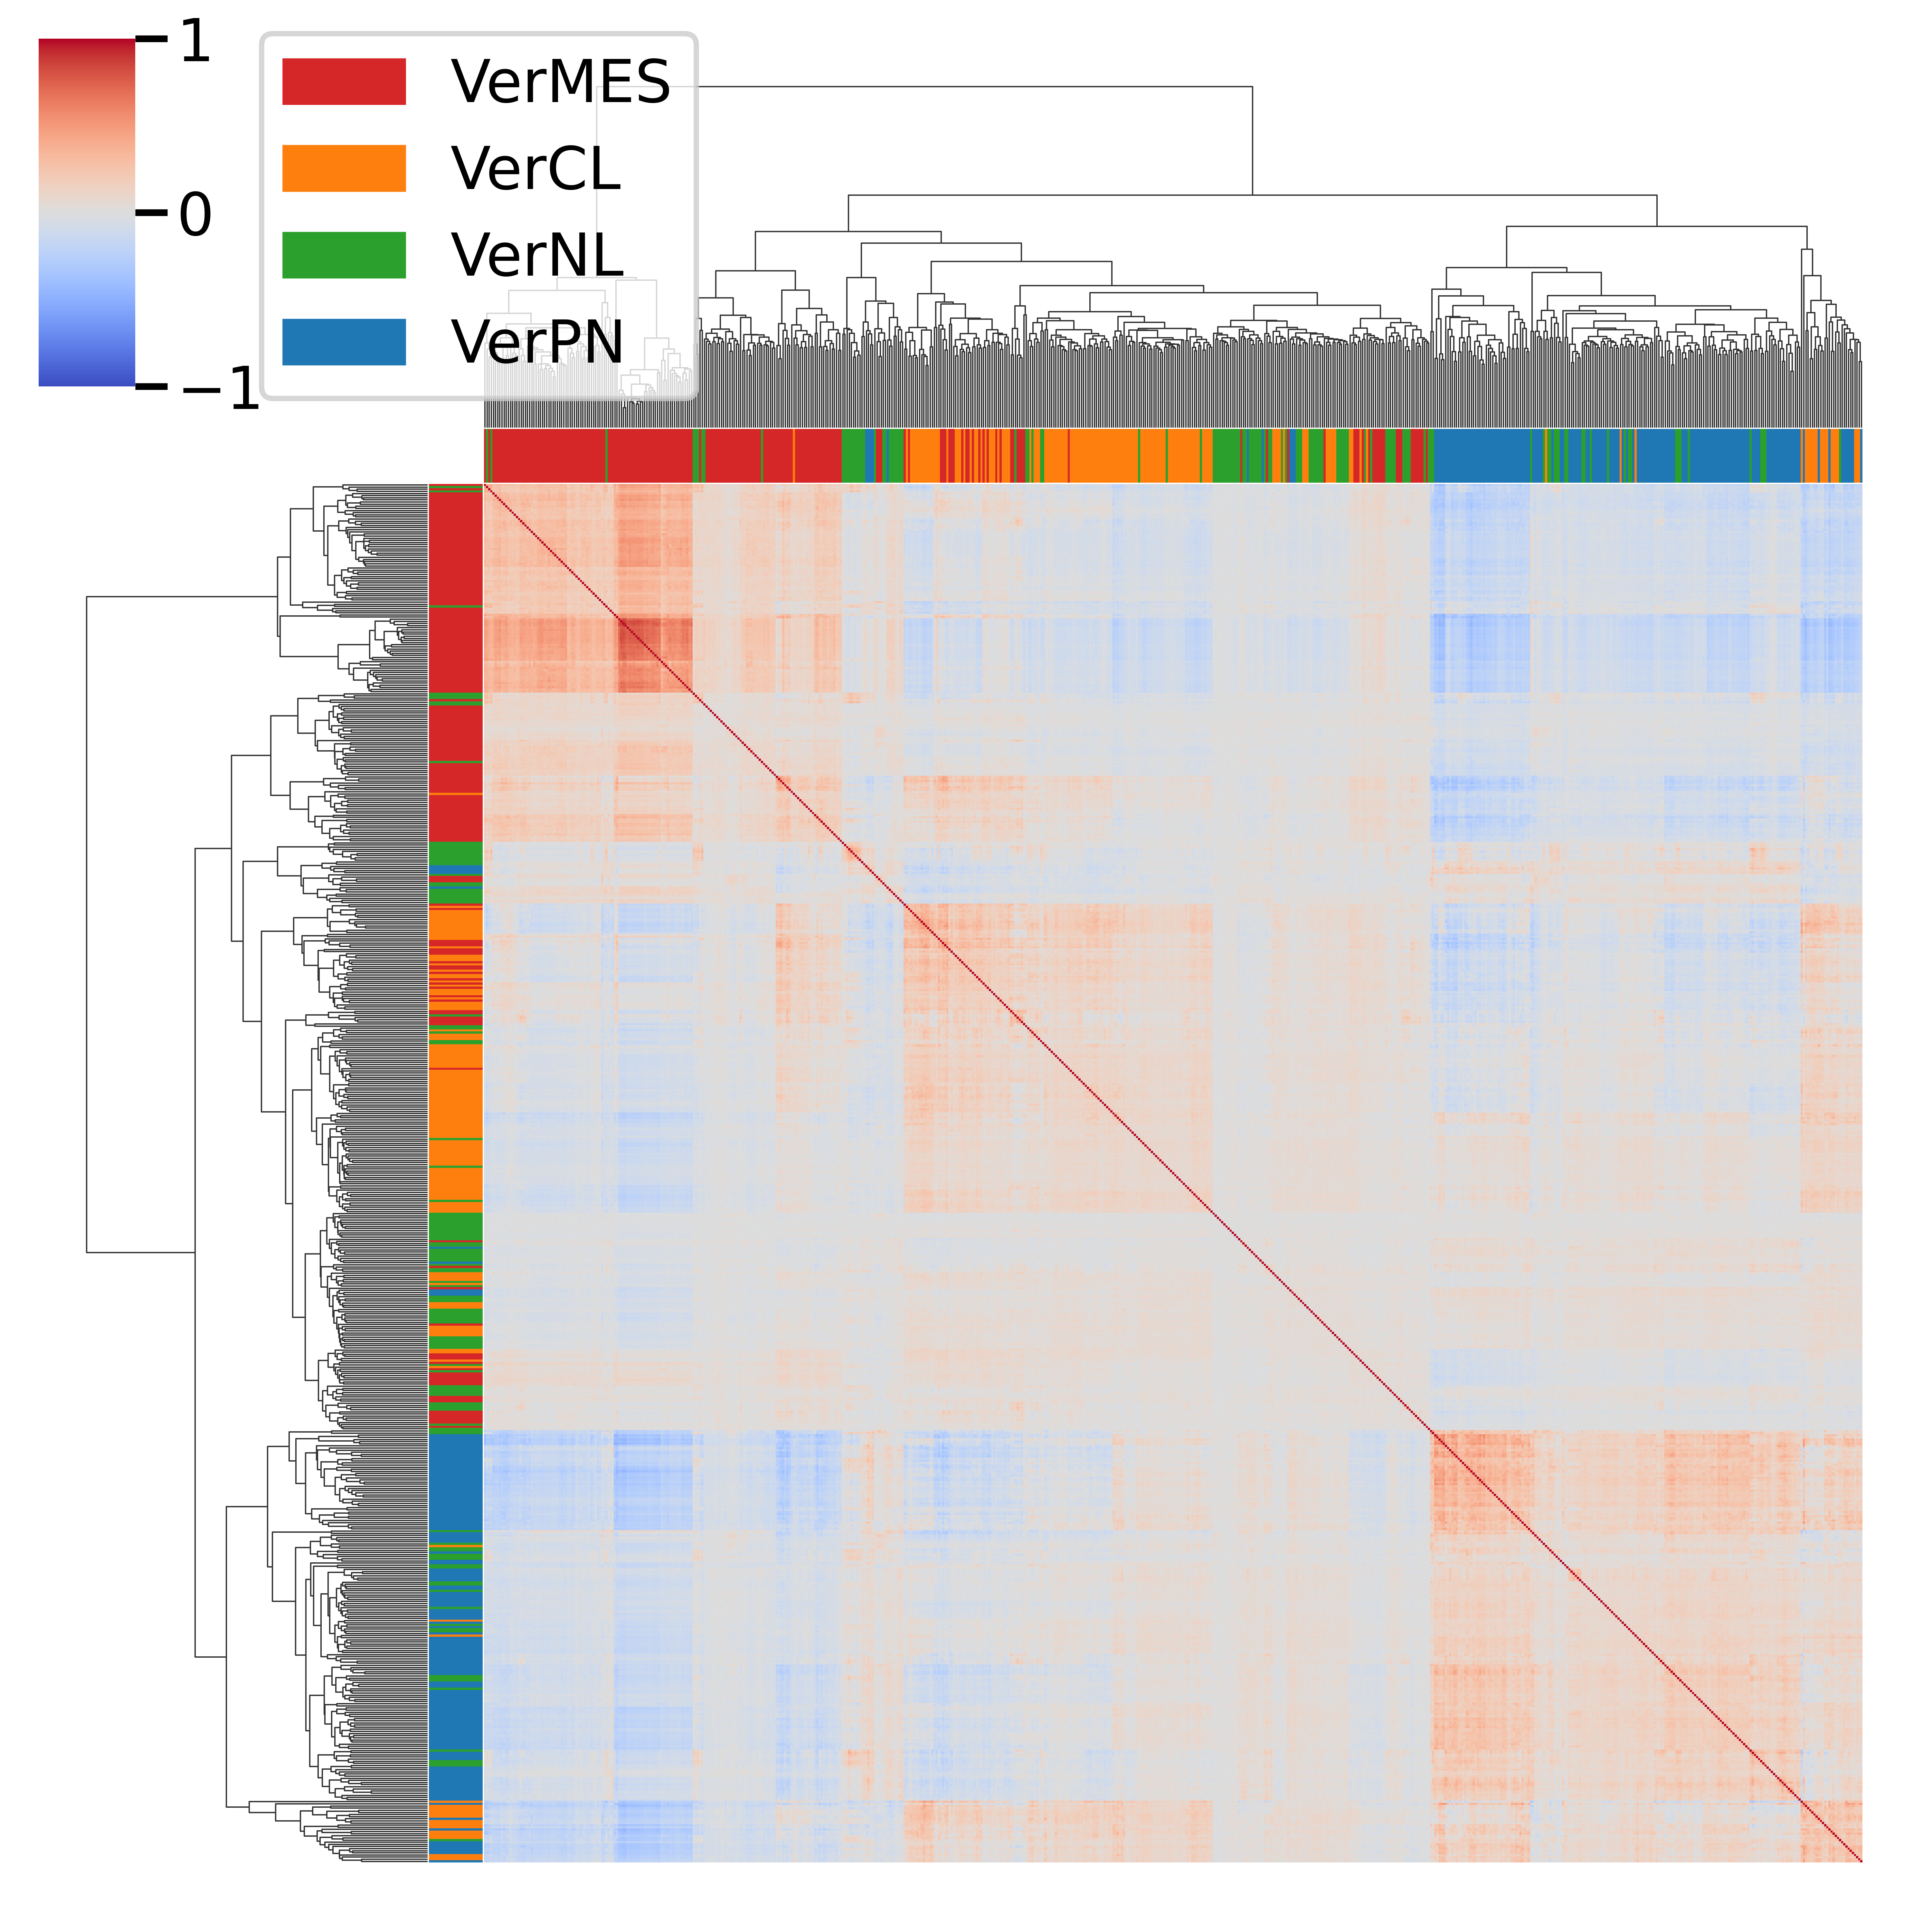
\includegraphics[width=\textwidth]{GSM3828672_Corrplot_Ver}
                    \caption{GSE131928}
                \end{subfigure}
                \begin{subfigure}[c]{0.48\textwidth}
                    \centering
                    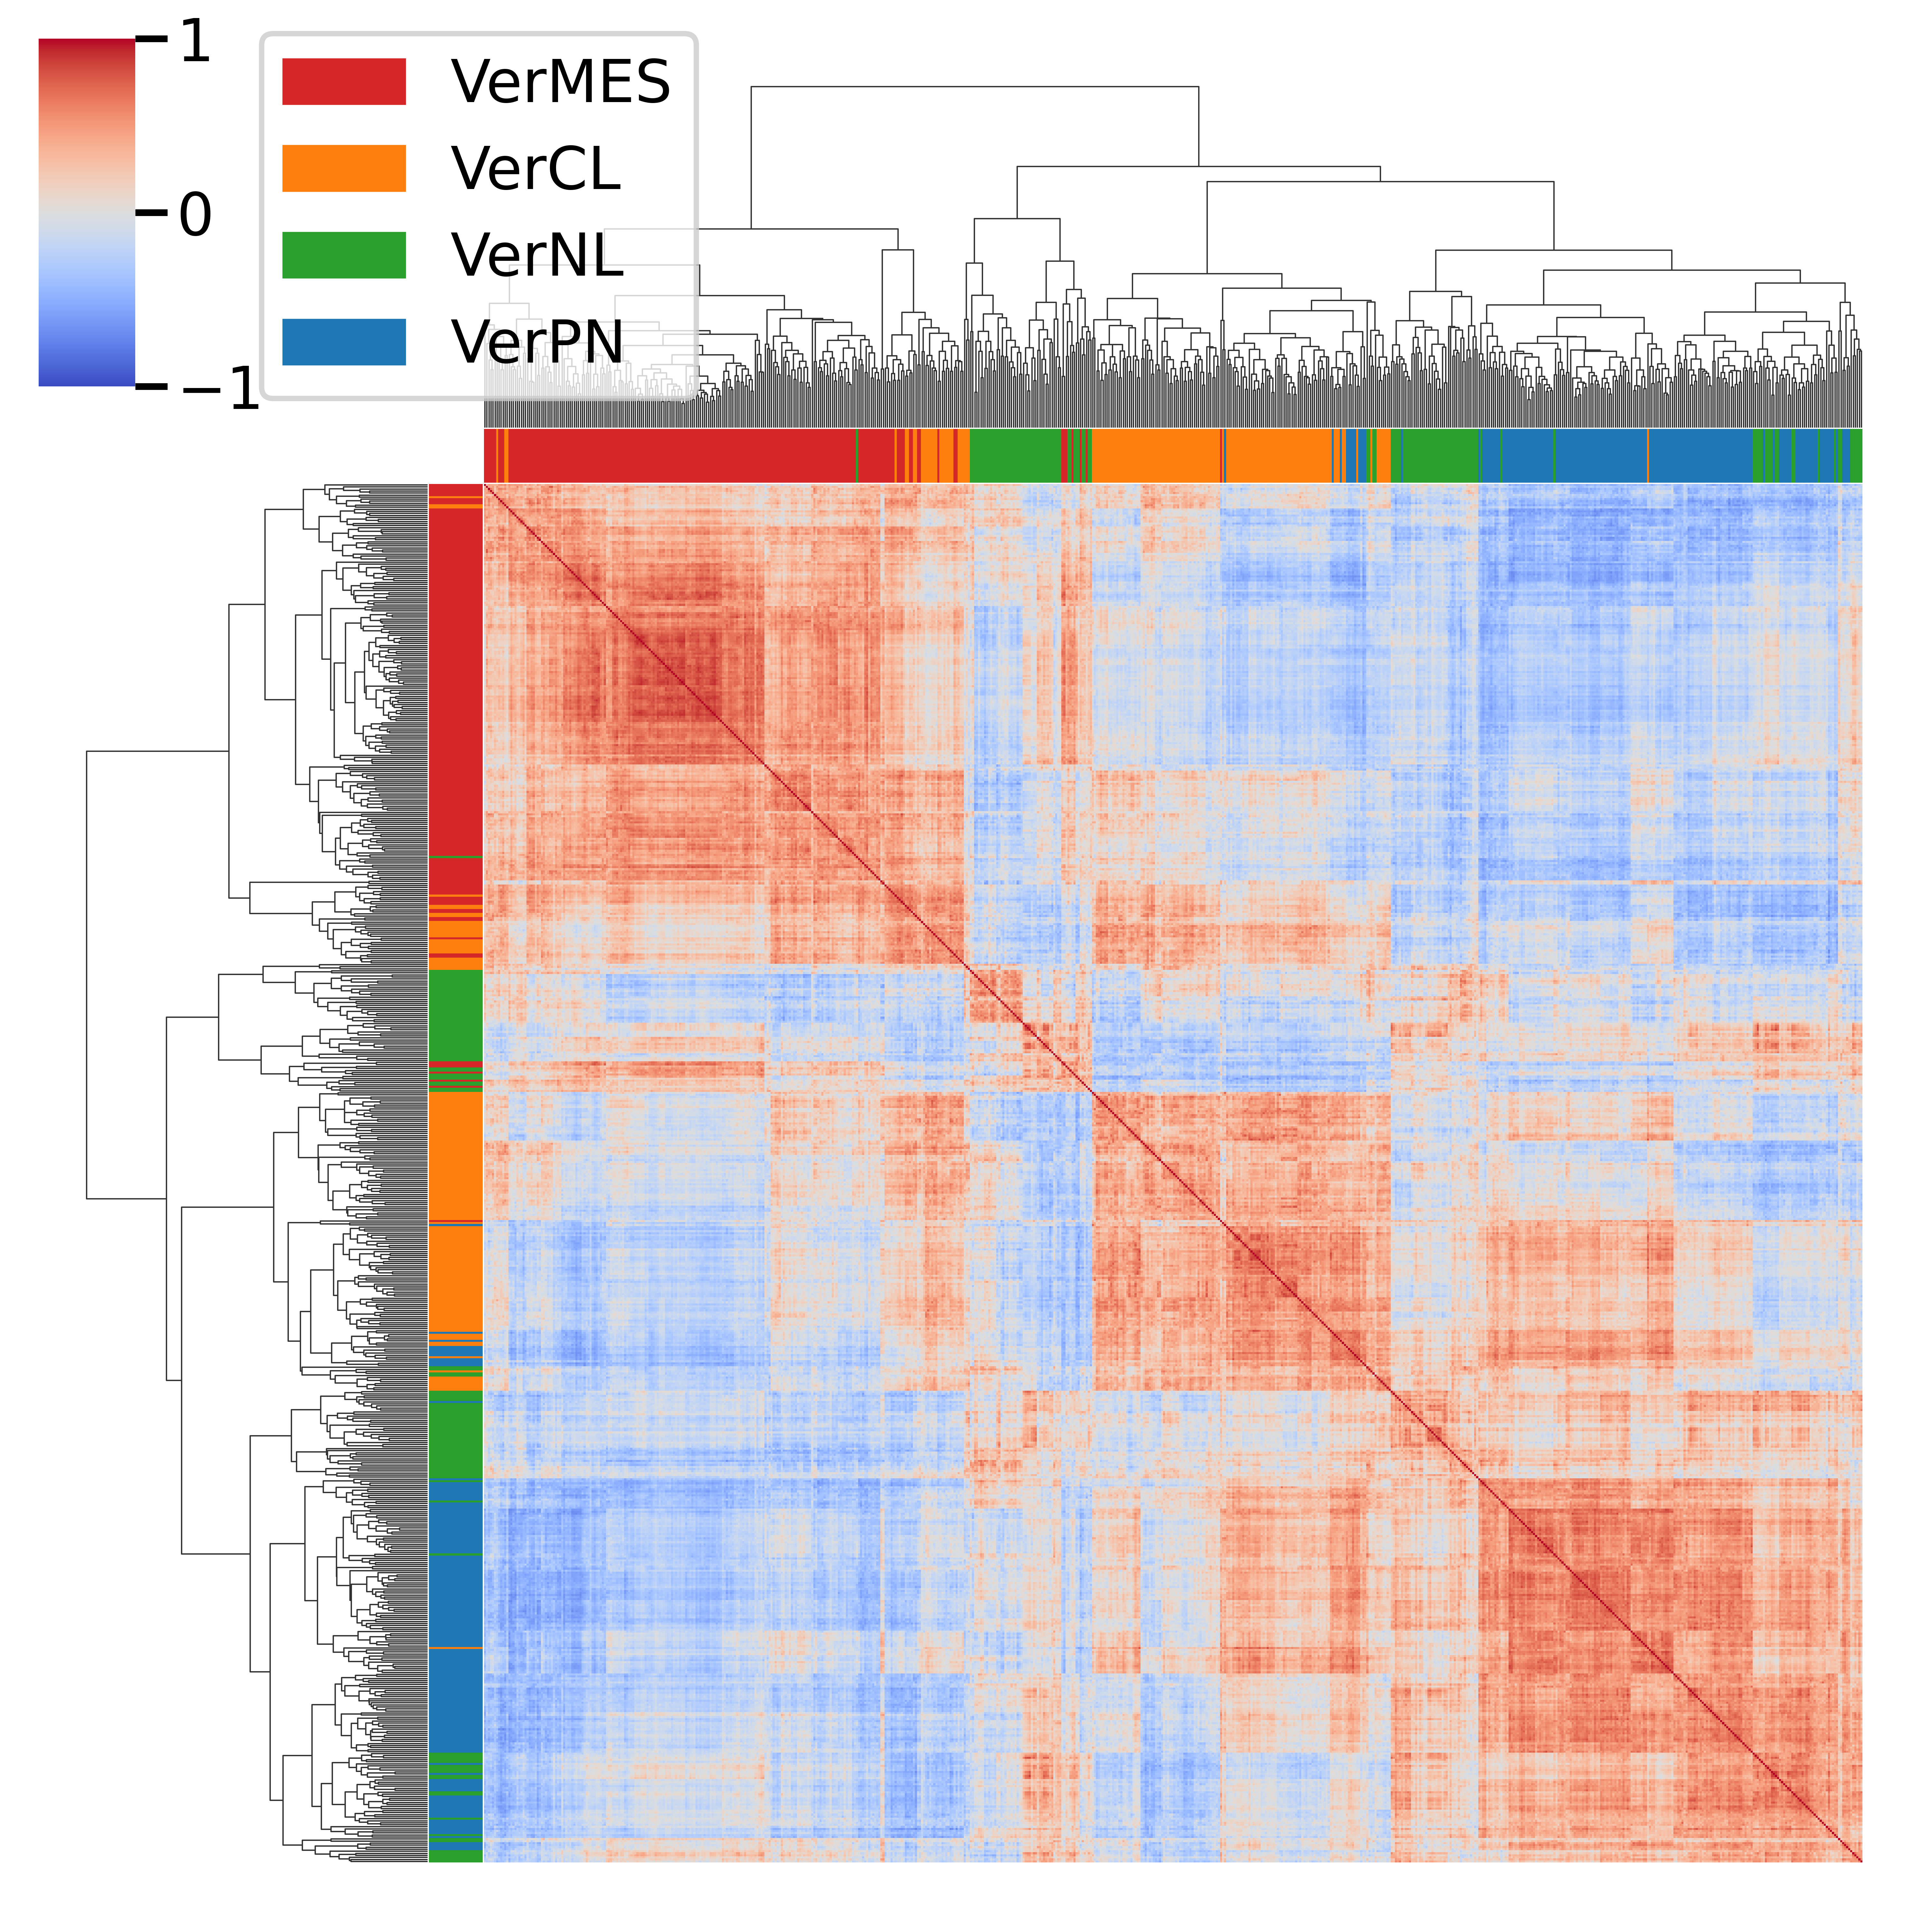
\includegraphics[width=\textwidth]{TCGA_Corrplot_Ver}
                    \caption{TCGA}
                \end{subfigure}
                \caption{Correlation of signature expression}
            \end{figure}
        \end{adjustwidth}
    \end{frame}

    \begin{frame}{Quantification of antagonism in correlation}
        \begin{columns}
            \begin{column}{0.55\textwidth}
                $$J = \underbrace{\sum_{x,y \in G_1} \frac{\rho_r(x,y)}{4 {N_1}^2} + \sum_{x,y \in G_2} \frac{\rho_r(x,y)}{4 {N_2}^2}}_{\text{Correlation within genesets}} - \underbrace{\sum_{x \in G_1, y \in G_2} \frac{\rho_r(x,y)}{2  N_1 N_2}}_{\text{Correlation across genesets}}$$
            \end{column}
            \begin{column}{0.45\textwidth}
                {\scriptsize Where,
                \begin{itemize}
                    \item $G_i =$ Gene Set i
                    \item $N_i =$ Number of genes in set i
                    \item $\rho_r(x,y) =$ Spearman correlation of gene x with gene y
                \end{itemize}}
            \end{column}
        \end{columns}
        \pause
        \begin{adjustwidth}{-5cm}{-5cm}
            \centering
            \begin{figure}
                \centering
                \begin{subfigure}[c]{0.27\textwidth}
                    \centering
                    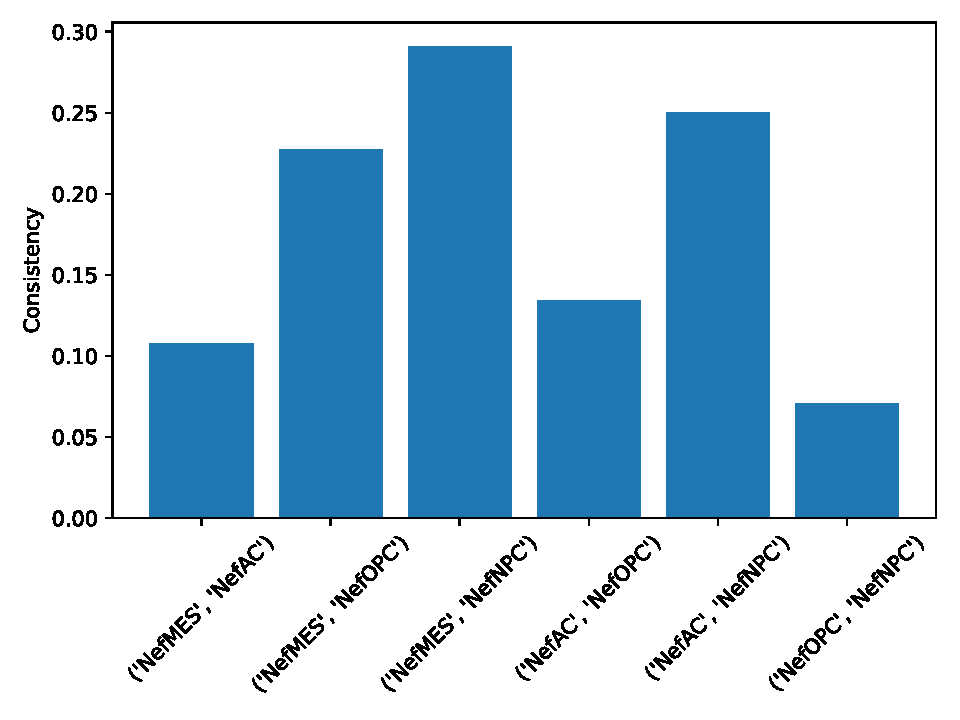
\includegraphics[width=\textwidth]{GSM3828672_Consistency_Nef}
                    \caption{GSE131928 - Neftel}
                \end{subfigure}
                \begin{subfigure}[c]{0.27\textwidth}
                    \centering
                    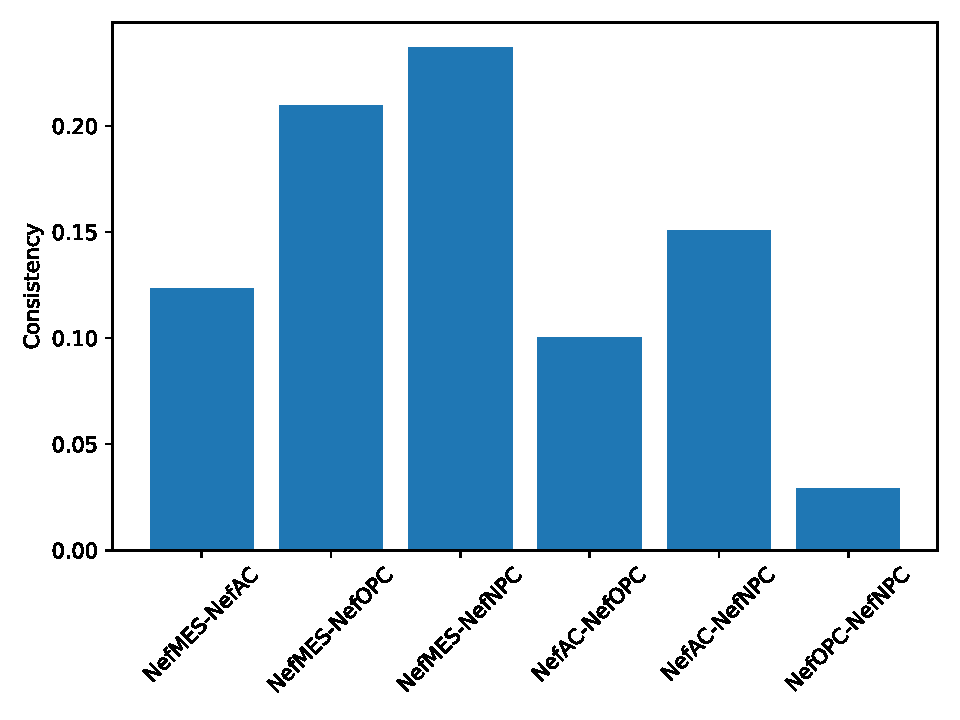
\includegraphics[width=\textwidth]{TCGA_Consistency_Nef}
                    \caption{TCGA - Neftel}
                \end{subfigure}
                \pause
                \begin{subfigure}[c]{0.27\textwidth}
                    \centering
                    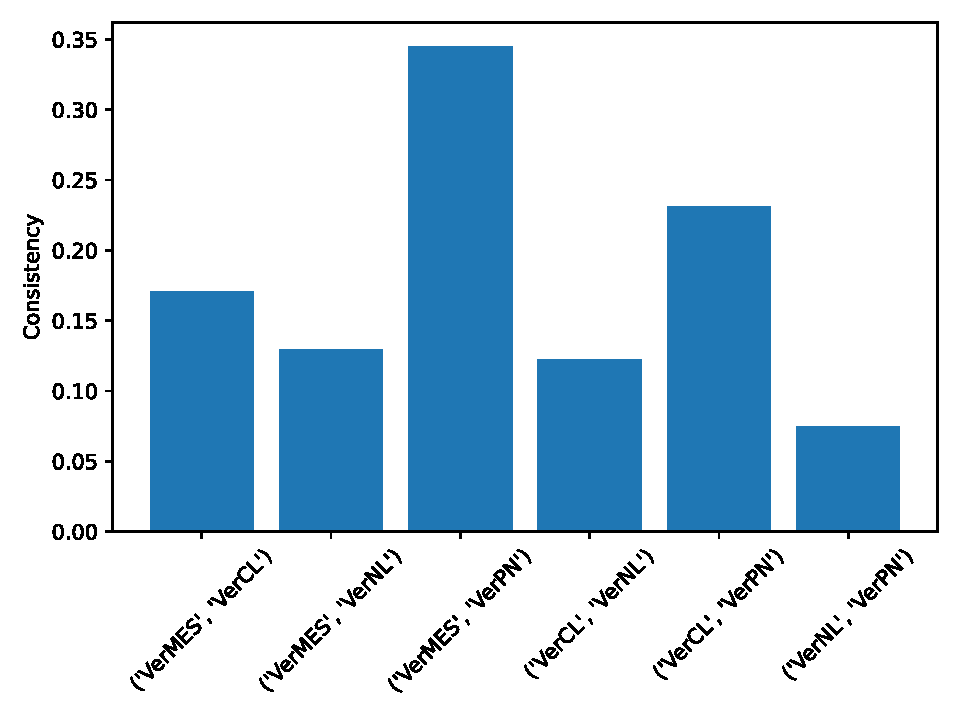
\includegraphics[width=\textwidth]{GSM3828672_Consistency_Ver}
                    \caption{GSE131928 - Verhaak}
                \end{subfigure}
                \begin{subfigure}[c]{0.27\textwidth}
                    \centering
                    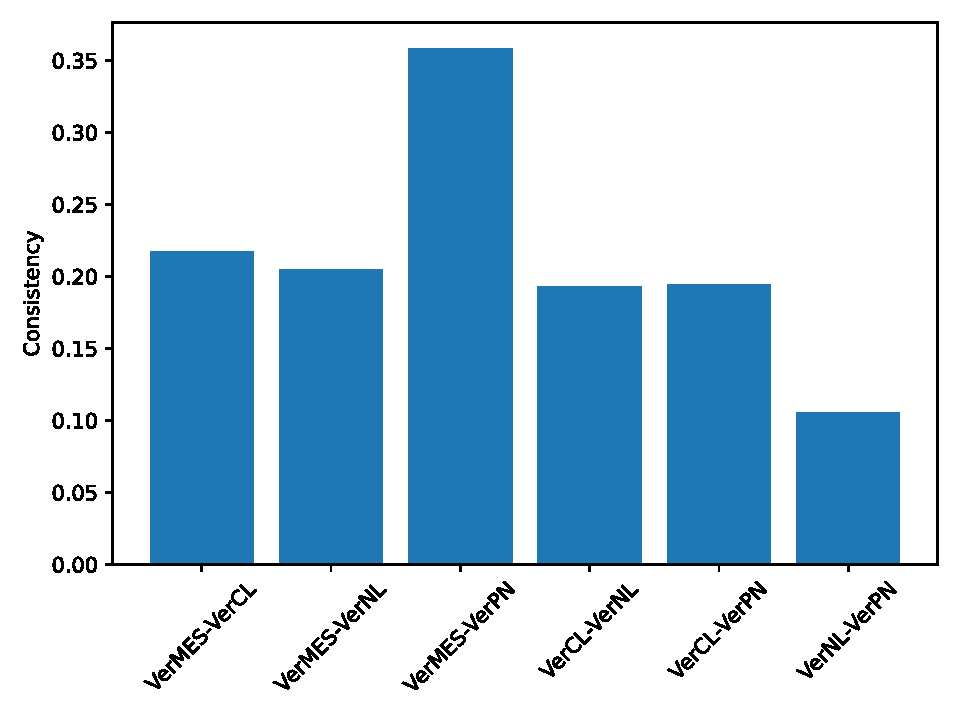
\includegraphics[width=\textwidth]{TCGA_Consistency_Ver}
                    \caption{TCGA - Verhaak}
                \end{subfigure}
            \pause[2]\caption{J metric of signature correlation}
            \end{figure}
        \end{adjustwidth}
    \end{frame}

    \begin{frame}{PC1 loadings are dominated by NPC-MES antagonism (Neftel)}
        \begin{adjustwidth}{-5cm}{-5cm}
            \centering
            \begin{figure}
                \centering
                \begin{subfigure}[c]{0.48\textwidth}
                    \centering
                    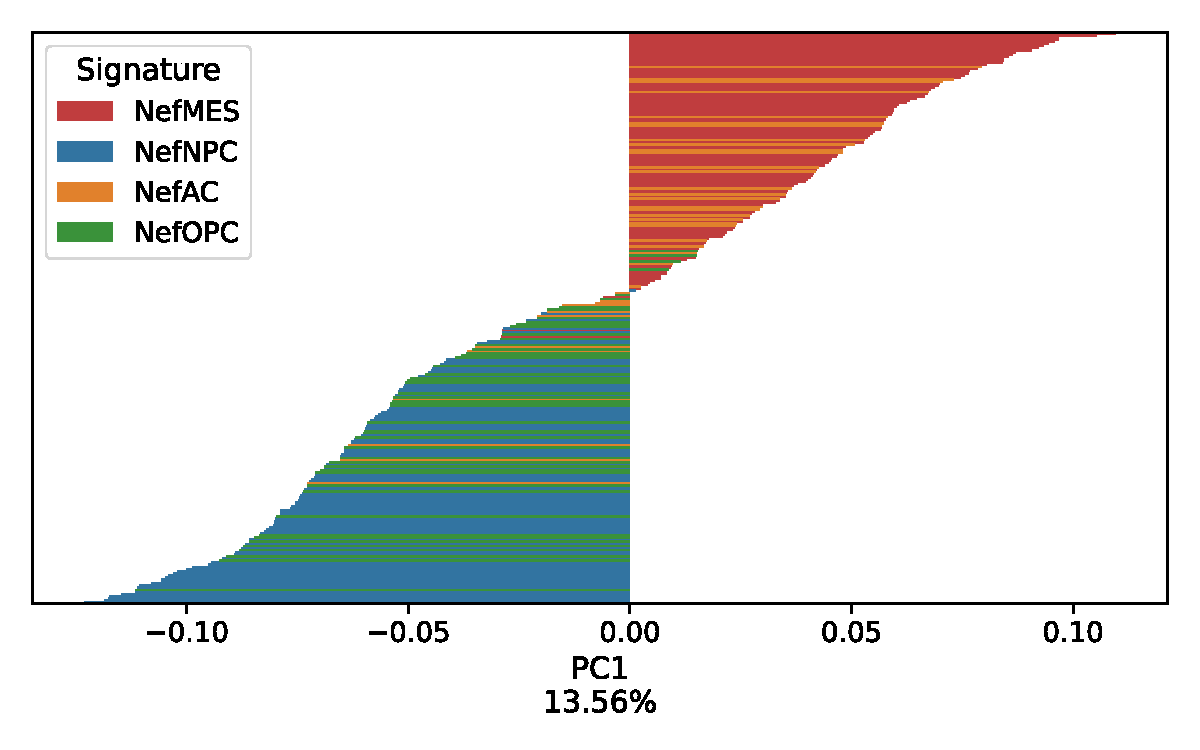
\includegraphics[width=\textwidth]{GSM3828672_loadingsPC1_barplot_Nef}
                    \caption{GSE131928}
                \end{subfigure}
                \begin{subfigure}[c]{0.48\textwidth}
                    \centering
                    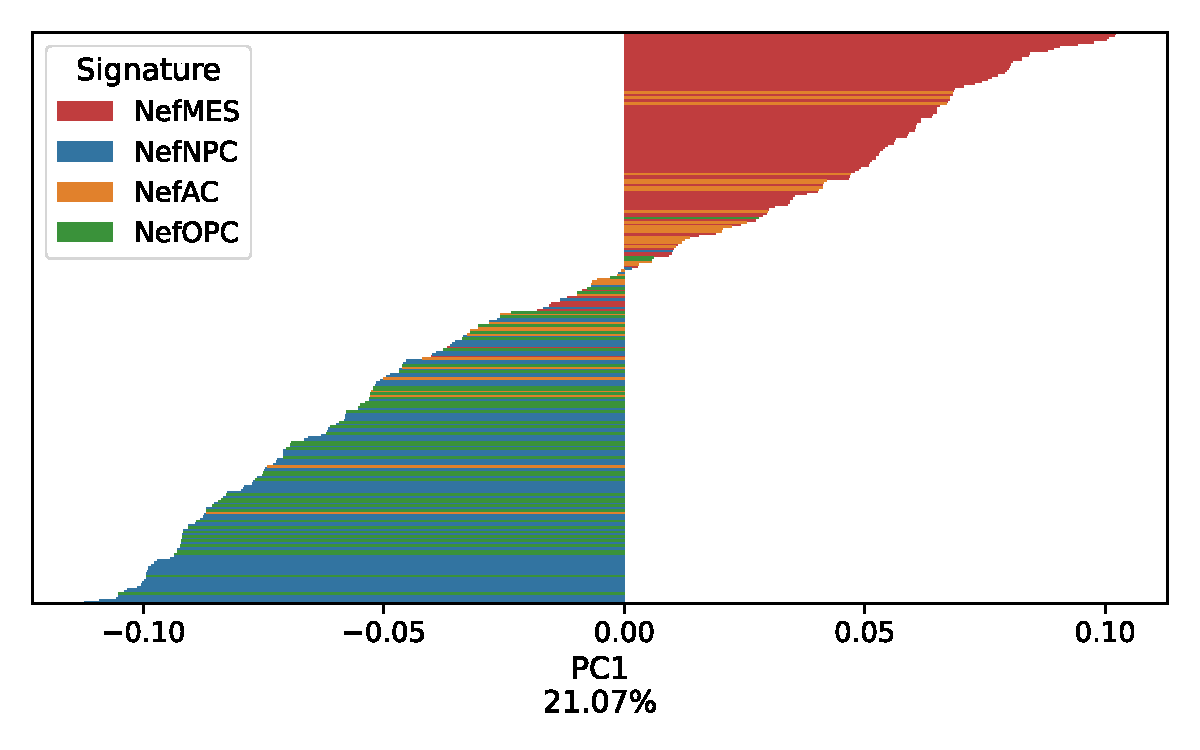
\includegraphics[width=\textwidth]{TCGA_loadingsPC1_barplot_Nef}
                    \caption{TCGA}
                \end{subfigure}
                \caption{PC1 loadings - PCA on signature expression}
            \end{figure}
        \end{adjustwidth}
    \end{frame}

    \begin{frame}{PC1 loadings are dominated by PN-MES antagonism (Verhaak)}
        \begin{adjustwidth}{-5cm}{-5cm}
            \centering
            \begin{figure}\ContinuedFloat
                \centering
                \begin{subfigure}[c]{0.48\textwidth}
                    \centering
                    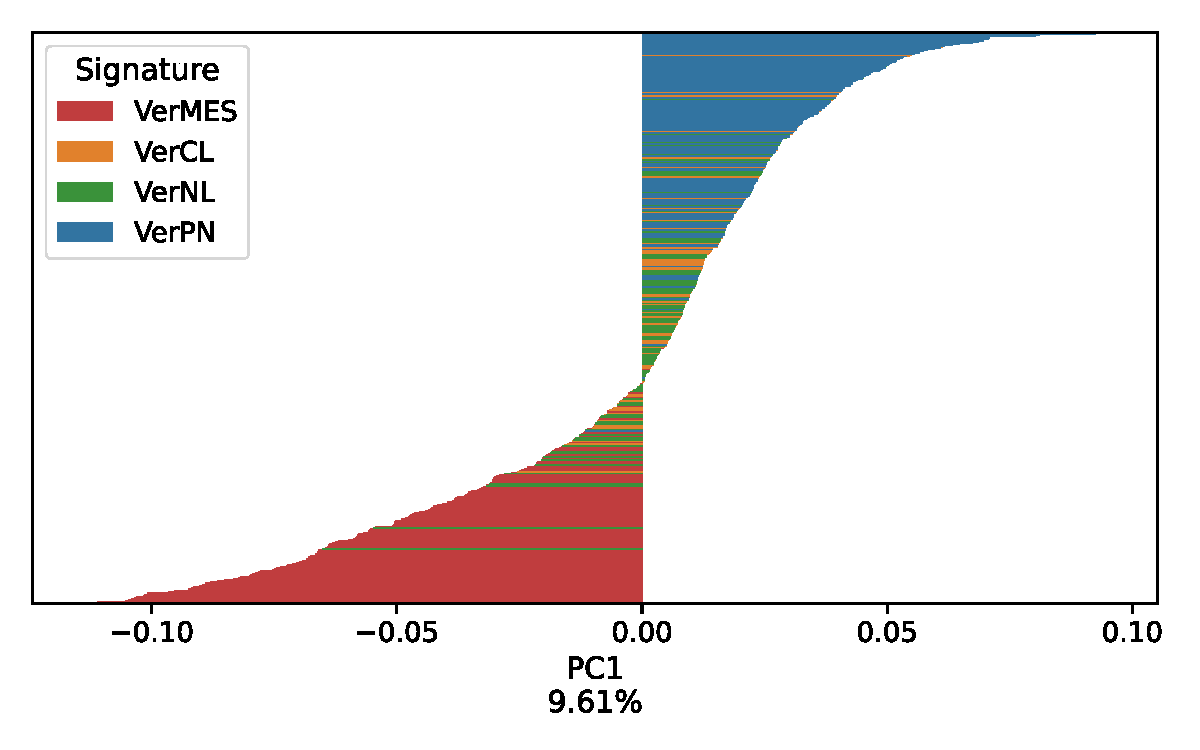
\includegraphics[width=\textwidth]{GSM3828672_loadingsPC1_barplot_Ver}
                    \caption{GSE131928}
                \end{subfigure}
                \begin{subfigure}[c]{0.48\textwidth}
                    \centering
                    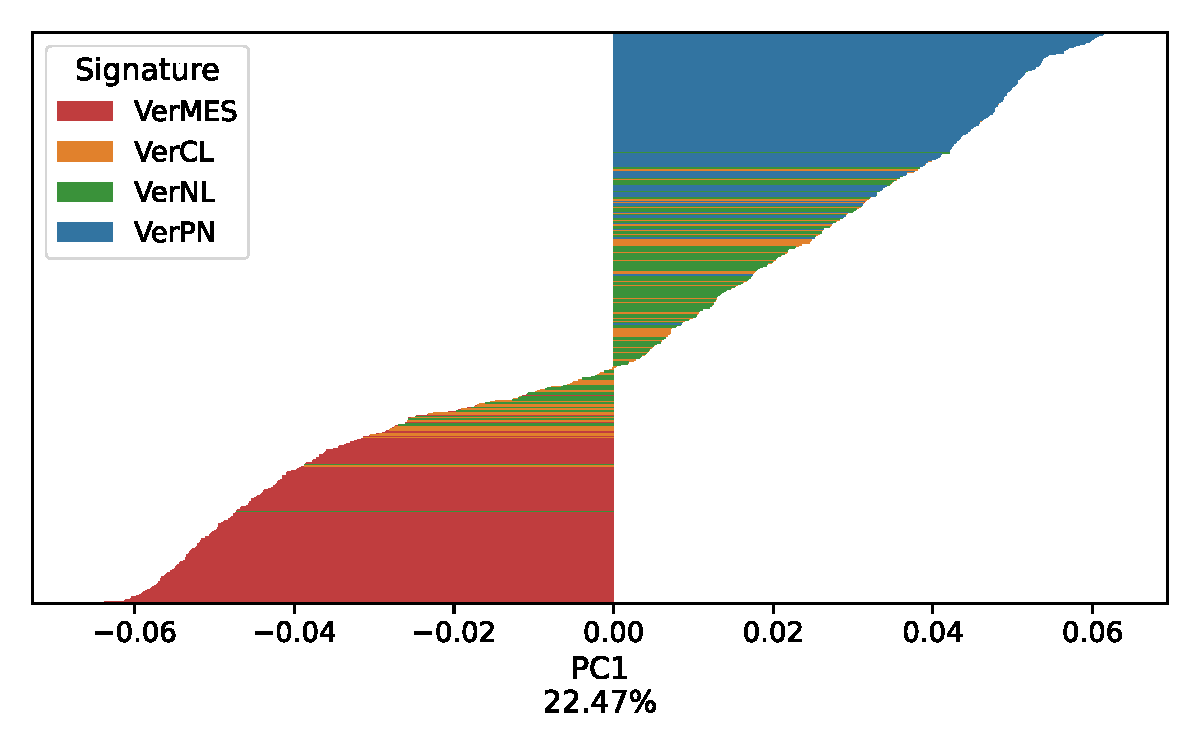
\includegraphics[width=\textwidth]{TCGA_loadingsPC1_barplot_Ver}
                    \caption{TCGA}
                \end{subfigure}
                \caption{PC1 loadings - PCA on signature expression}
            \end{figure}
        \end{adjustwidth}
    \end{frame}

%     \begin{frame}{PC2 loadings does not segregate AC-OPC (Verhaak)}
%     \end{frame}
%     \begin{frame}{PC2 loadings segregate CL-NL (Verhaak)}
%     \end{frame}

    % \begin{frame}{Signatures}
    %     \begin{adjustwidth}{-5cm}{-5cm}
    %         \centering
    %         \begin{figure}
    %             \centering
    %             \begin{subfigure}[c]{0.38\textwidth}
    %                 \centering
    %                 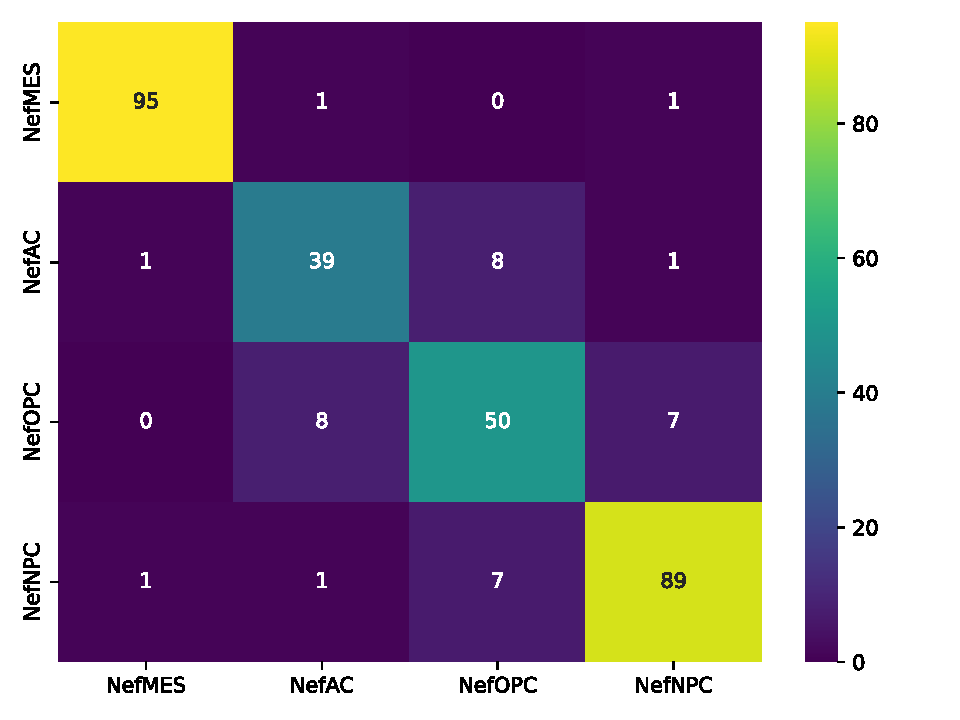
\includegraphics[width=\textwidth]{signature_overlap_Nef}
    %                 \caption{Neftel et al signature}
    %             \end{subfigure}
    %             \pause
    %             \begin{subfigure}[c]{0.38\textwidth}
    %                 \centering
    %                 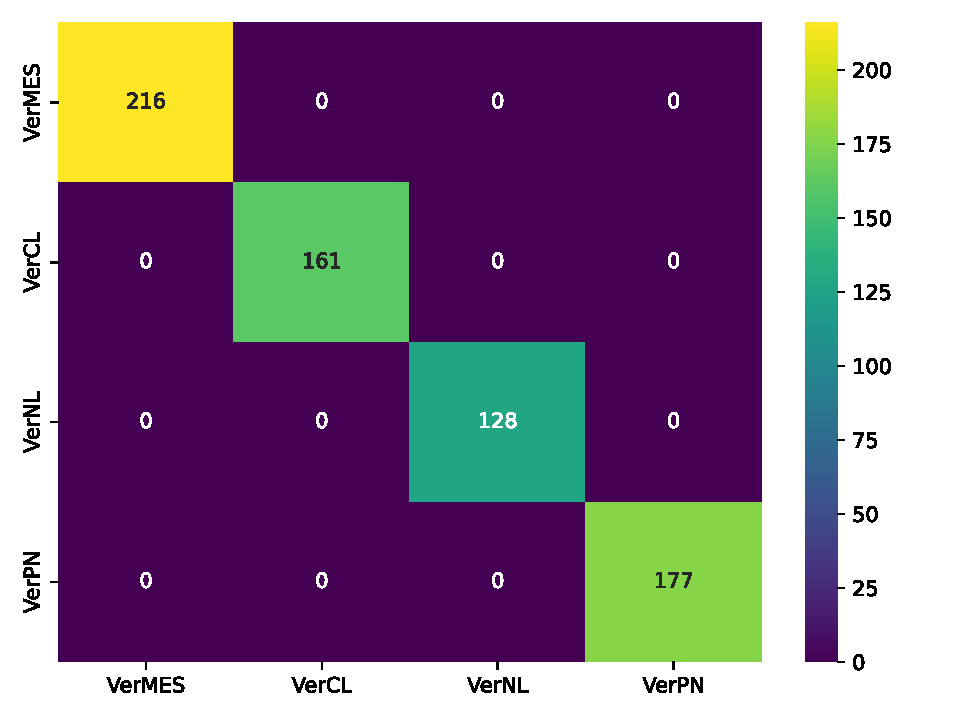
\includegraphics[width=\textwidth]{signature_overlap_Ver}
    %                 \caption{Verhaak et al signature}
    %             \end{subfigure}
    %             \pause
    %             \begin{subfigure}[c]{0.38\textwidth}
    %                 \centering
    %                 \includegraphics[width=\textwidth]{signature_overlap_All}
    %                 \caption{Signature of both}
    %             \end{subfigure}
    %             \pause[1]\caption{Overlap of genes in the signatures}
    %         \end{figure}
    %     \end{adjustwidth}
    % \end{frame}

    \begin{frame}{Observed trend holds across multiple Bulk RNASeq datasets}
        \begin{adjustwidth}{-5cm}{-5cm}
            \centering
            \begin{figure}
                \centering
                \begin{subfigure}[c]{0.22\textwidth}
                    \centering
                    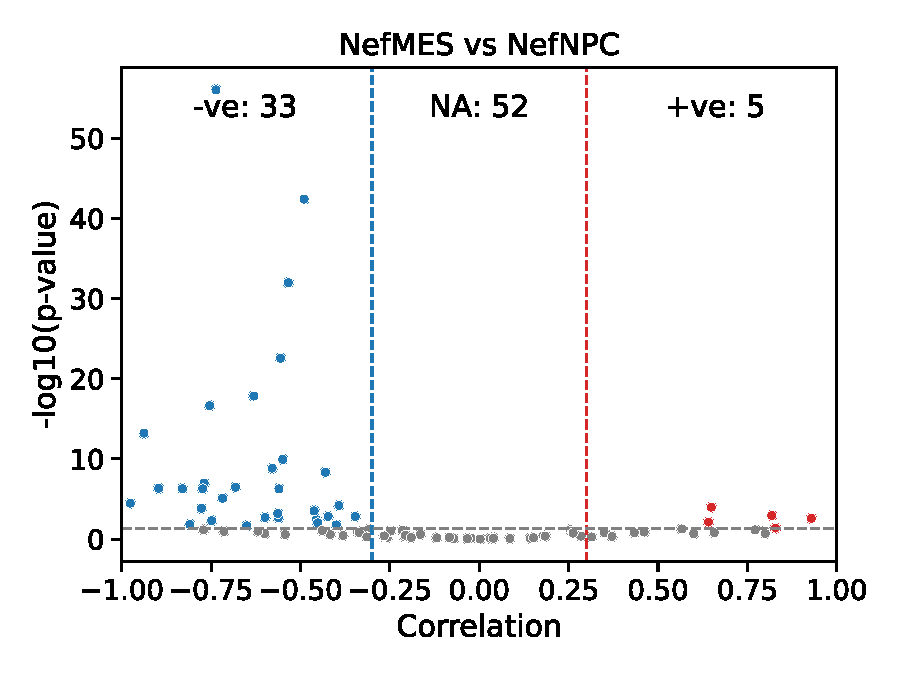
\includegraphics[width=\textwidth]{Volcano_Bulk_NefMES-NefNPC}
                \end{subfigure}
                \begin{subfigure}[c]{0.33\textwidth}
                    \centering
                    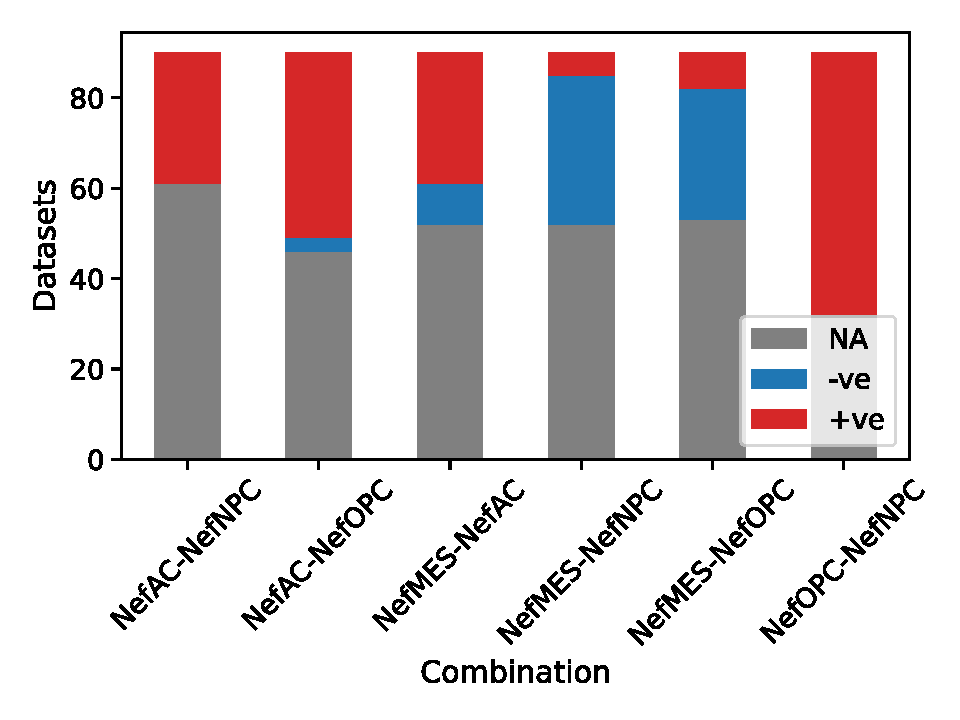
\includegraphics[width=\textwidth]{Bar_Bulk_Nef}
                    \caption{Neftel}
                \end{subfigure}
                \pause
                \begin{subfigure}[c]{0.22\textwidth}
                    \centering
                    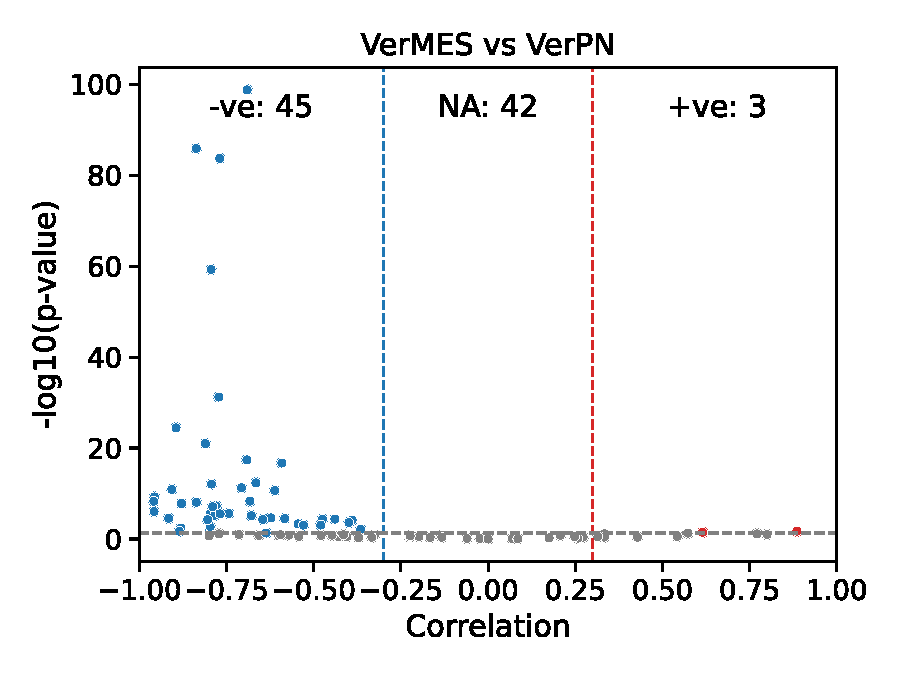
\includegraphics[width=\textwidth]{Volcano_Bulk_VerMES-VerPN}
                \end{subfigure}
                \begin{subfigure}[c]{0.33\textwidth}
                    \centering
                    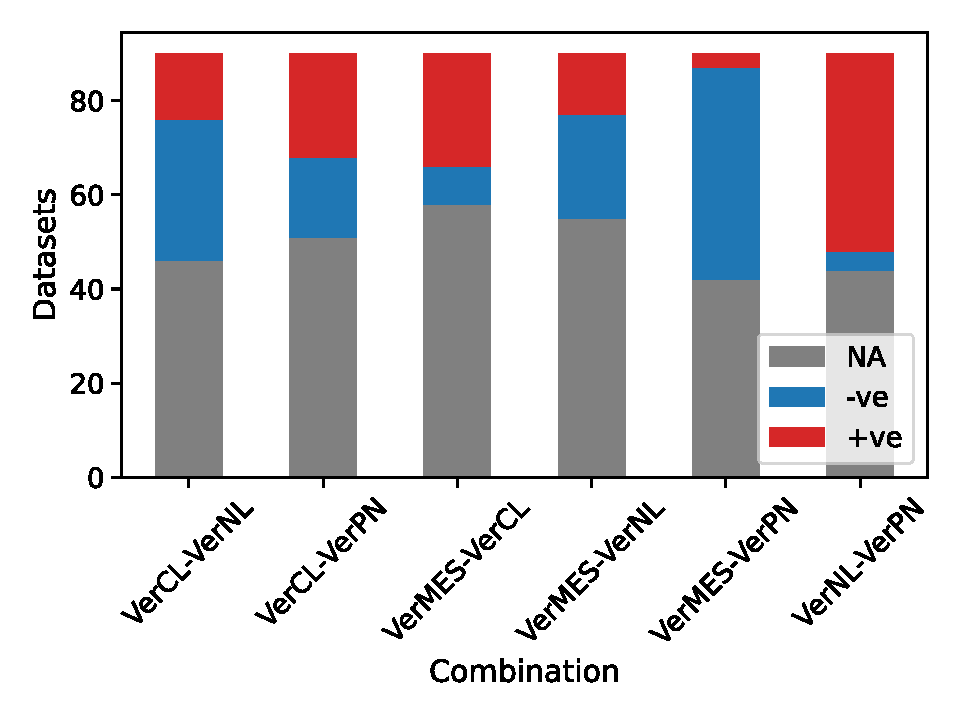
\includegraphics[width=\textwidth]{Bar_Bulk_Ver}
                    \caption{Verhaak}
                \end{subfigure}
                \pause[1]\caption{Metanalysis of Bulk datasets}
            \end{figure}
        \end{adjustwidth}
    \end{frame}

    \begin{frame}{Observed trend holds across multiple SingleCell RNASeq datasets}
        \begin{adjustwidth}{-5cm}{-5cm}
            \centering
            \begin{figure}\ContinuedFloat
                \centering
                \begin{subfigure}[c]{0.22\textwidth}
                    \centering
                    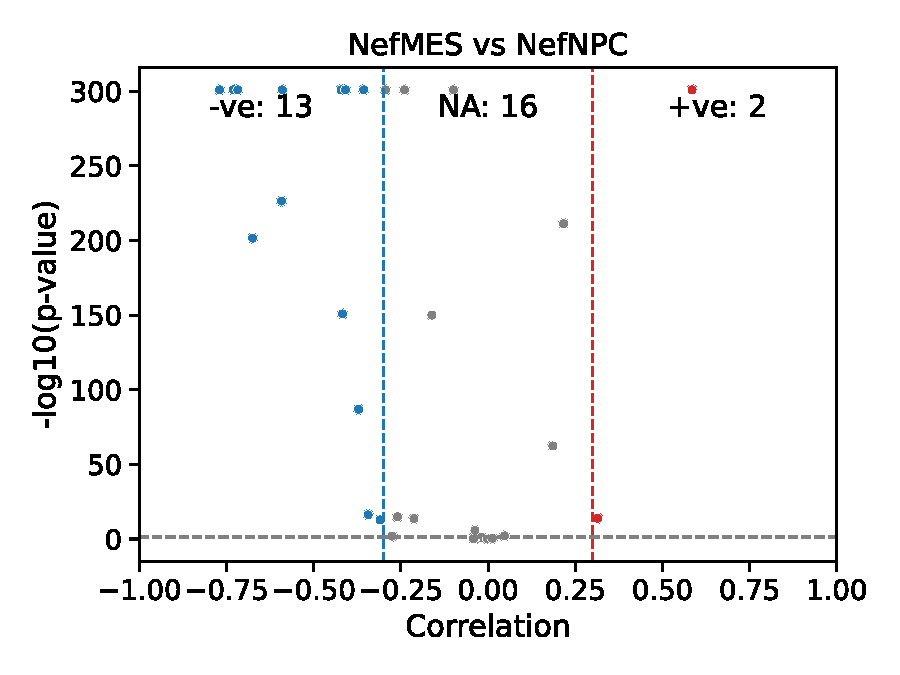
\includegraphics[width=\textwidth]{Volcano_SC_NefMES-NefNPC}
                \end{subfigure}
                \begin{subfigure}[c]{0.33\textwidth}
                    \centering
                    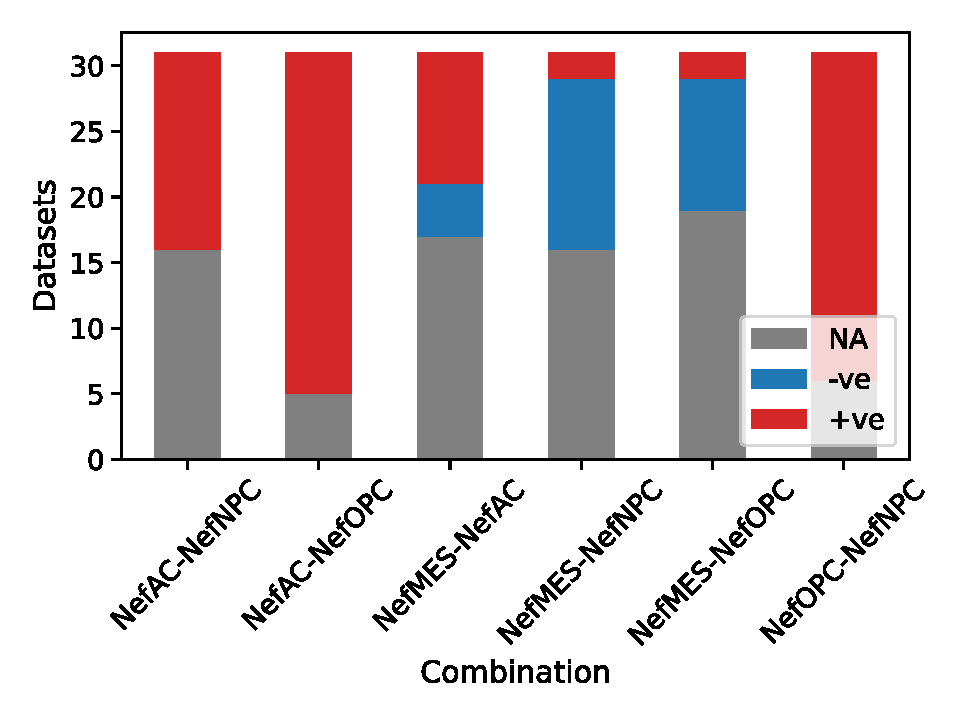
\includegraphics[width=\textwidth]{Bar_SC_Nef}
                    \caption{Neftel}
                \end{subfigure}
                \pause
                \begin{subfigure}[c]{0.22\textwidth}
                    \centering
                    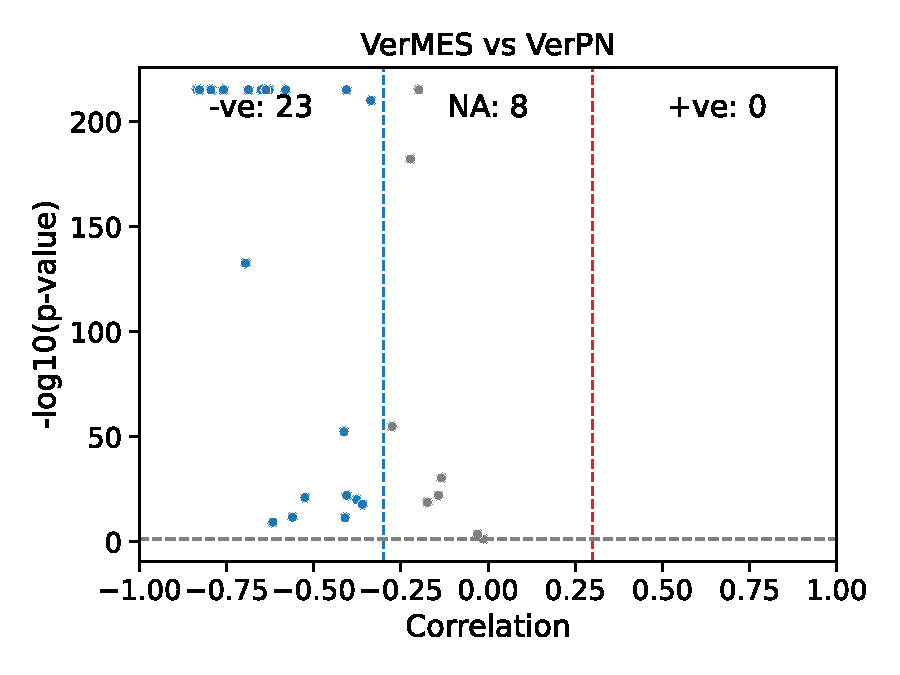
\includegraphics[width=\textwidth]{Volcano_SC_VerMES-VerPN}
                \end{subfigure}
                \begin{subfigure}[c]{0.33\textwidth}
                    \centering
                    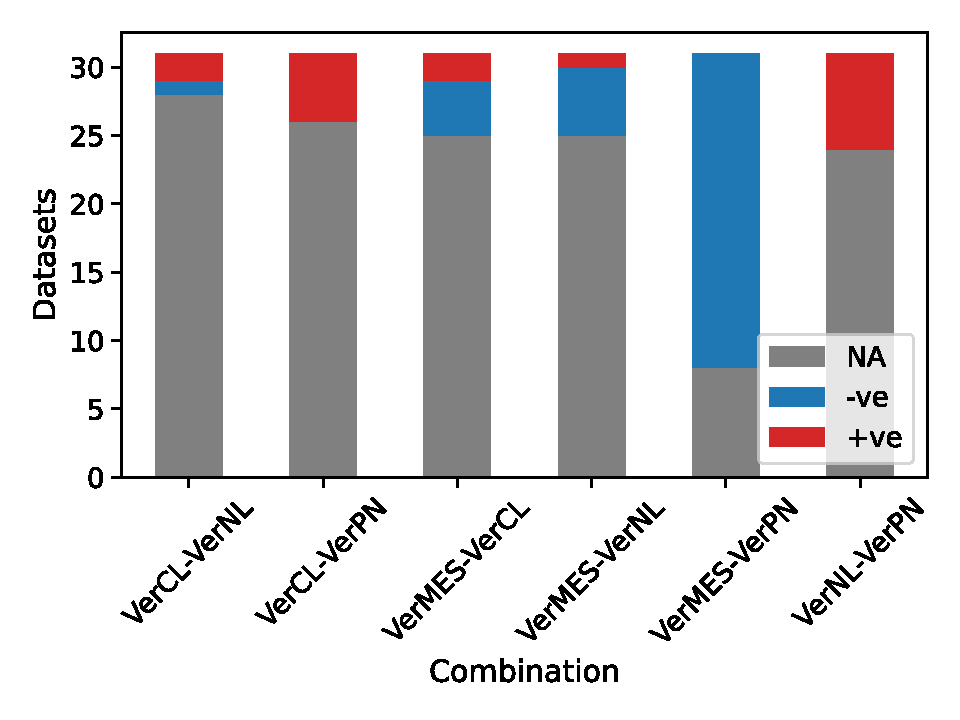
\includegraphics[width=\textwidth]{Bar_SC_Ver}
                    \caption{Verhaak}
                \end{subfigure}
                \pause[1]\caption{Metanalysis of SingleCell datasets}
            \end{figure}
        \end{adjustwidth}
    \end{frame}

    \begin{frame}{Trends are consistent in Metabolic and Immune axis}
        \begin{adjustwidth}{-5cm}{-5cm}
            \centering
            \begin{figure}
                \centering
                \begin{subfigure}[c]{0.27\textwidth}
                    \centering
                    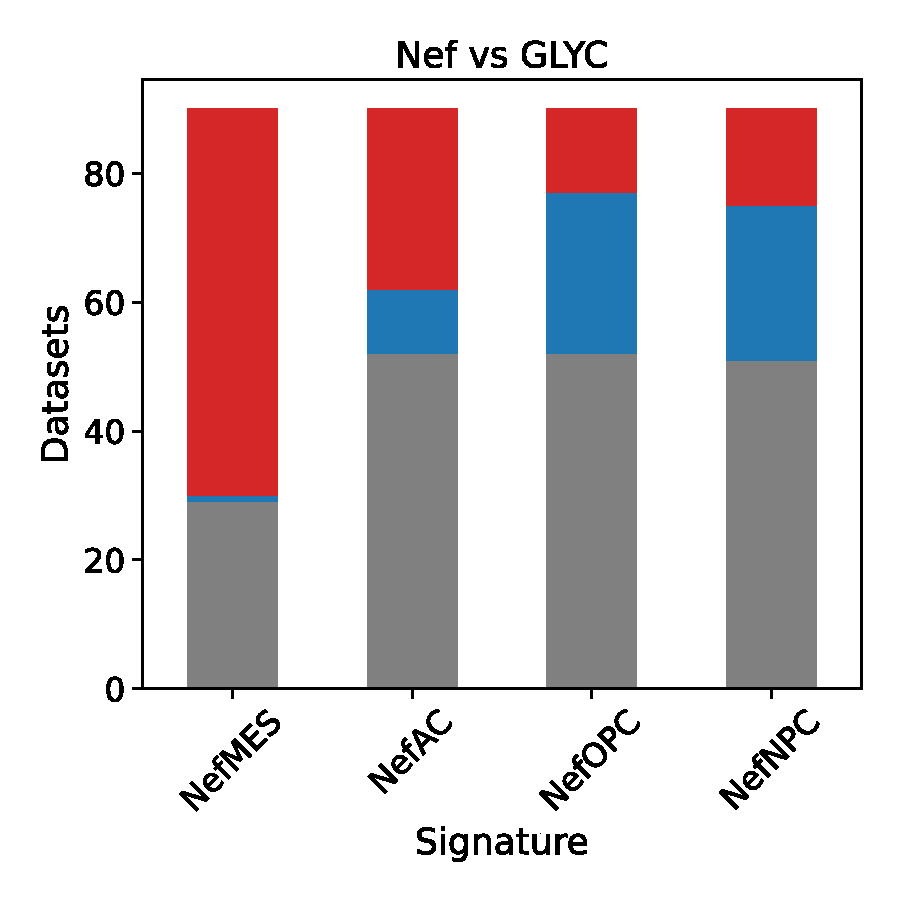
\includegraphics[width=\textwidth]{Bar_Bulk_Nef-GLYC}
                    \caption{Neftel - Glycolysis}
                \end{subfigure}
                \begin{subfigure}[c]{0.27\textwidth}
                    \centering
                    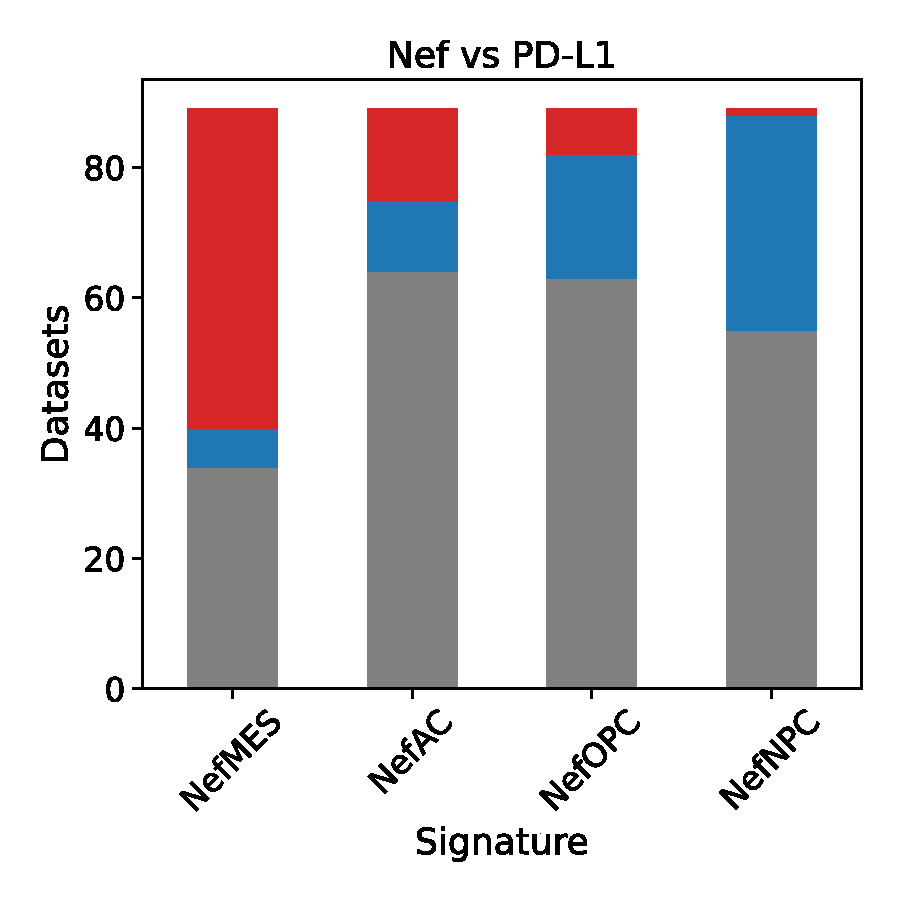
\includegraphics[width=\textwidth]{Bar_Bulk_Nef-PD-L1}
                    \caption{Neftel - PD-L1}
                \end{subfigure}
                \pause
                \begin{subfigure}[c]{0.27\textwidth}
                    \centering
                    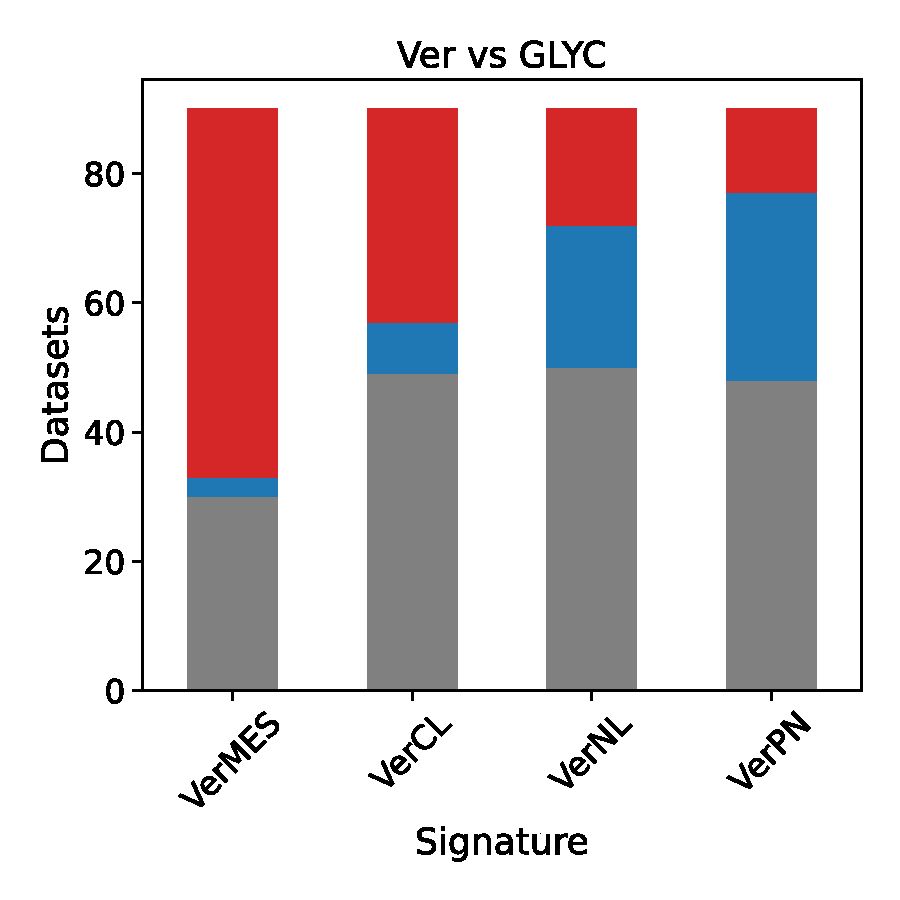
\includegraphics[width=\textwidth]{Bar_Bulk_Ver-GLYC}
                    \caption{Verhaak - Glycolysis}
                \end{subfigure}
                \begin{subfigure}[c]{0.27\textwidth}
                    \centering
                    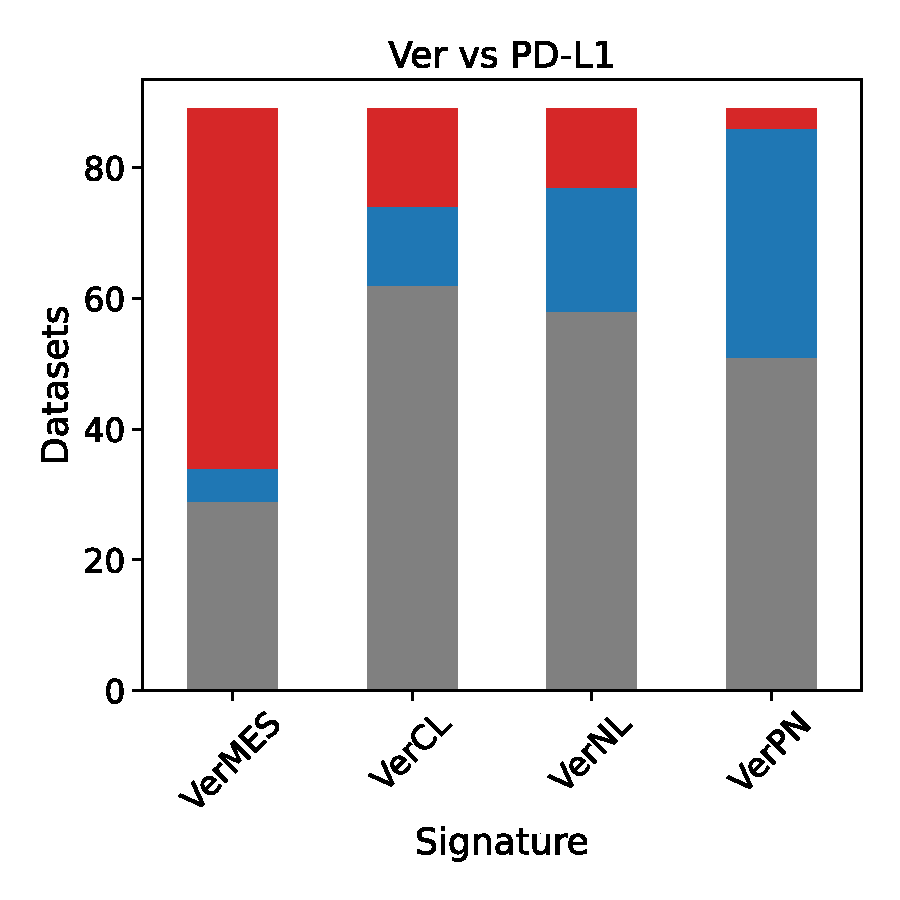
\includegraphics[width=\textwidth]{Bar_Bulk_Ver-PD-L1}
                    \caption{Verhaak - PD-L1}
                \end{subfigure}
                \pause[1]\caption{Correlation of subtypes with metabolism/immune axis}
            \end{figure}
        \end{adjustwidth}
    \end{frame}

%     \section{Conclusion}

    \begin{frame}{Conclusion}
        \begin{itemize}
            \item We can't find the 4 states mentioned in Neftel or Verhaak to be distinct
            \pause \item Most antagonistic pair
            \begin{itemize}
                \item NPC vs MES - Neftel et al
                \item PN vs MES - Verhaak et al
            \end{itemize}
            \pause \item NPC/PN - MES classification should be given more focus for therapeutic targetting efforts
            \begin{itemize}
                \item Targetting similar states (NPC-OPC) can give similar response to differing degree
                \item Targetting antagonistic states (NPC-MES) can give opposing response
            \end{itemize}
        \end{itemize}
    \end{frame}

    \begin{frame}{Future work}
        \begin{itemize}
            \item Why do we observe these trends? Can we explain them mechanistically?
            \pause
            \begin{itemize}
                \item Contruct a Gene regulatory network
            \end{itemize}
            \pause
            \item Strengthen the argument across multiple regulatory levels
        \end{itemize}
    \end{frame}

    \begin{frame}{Acknowledgements}
    \begin{columns}
        \begin{column}{0.65\textwidth}
        \begin{figure}
            \centering
            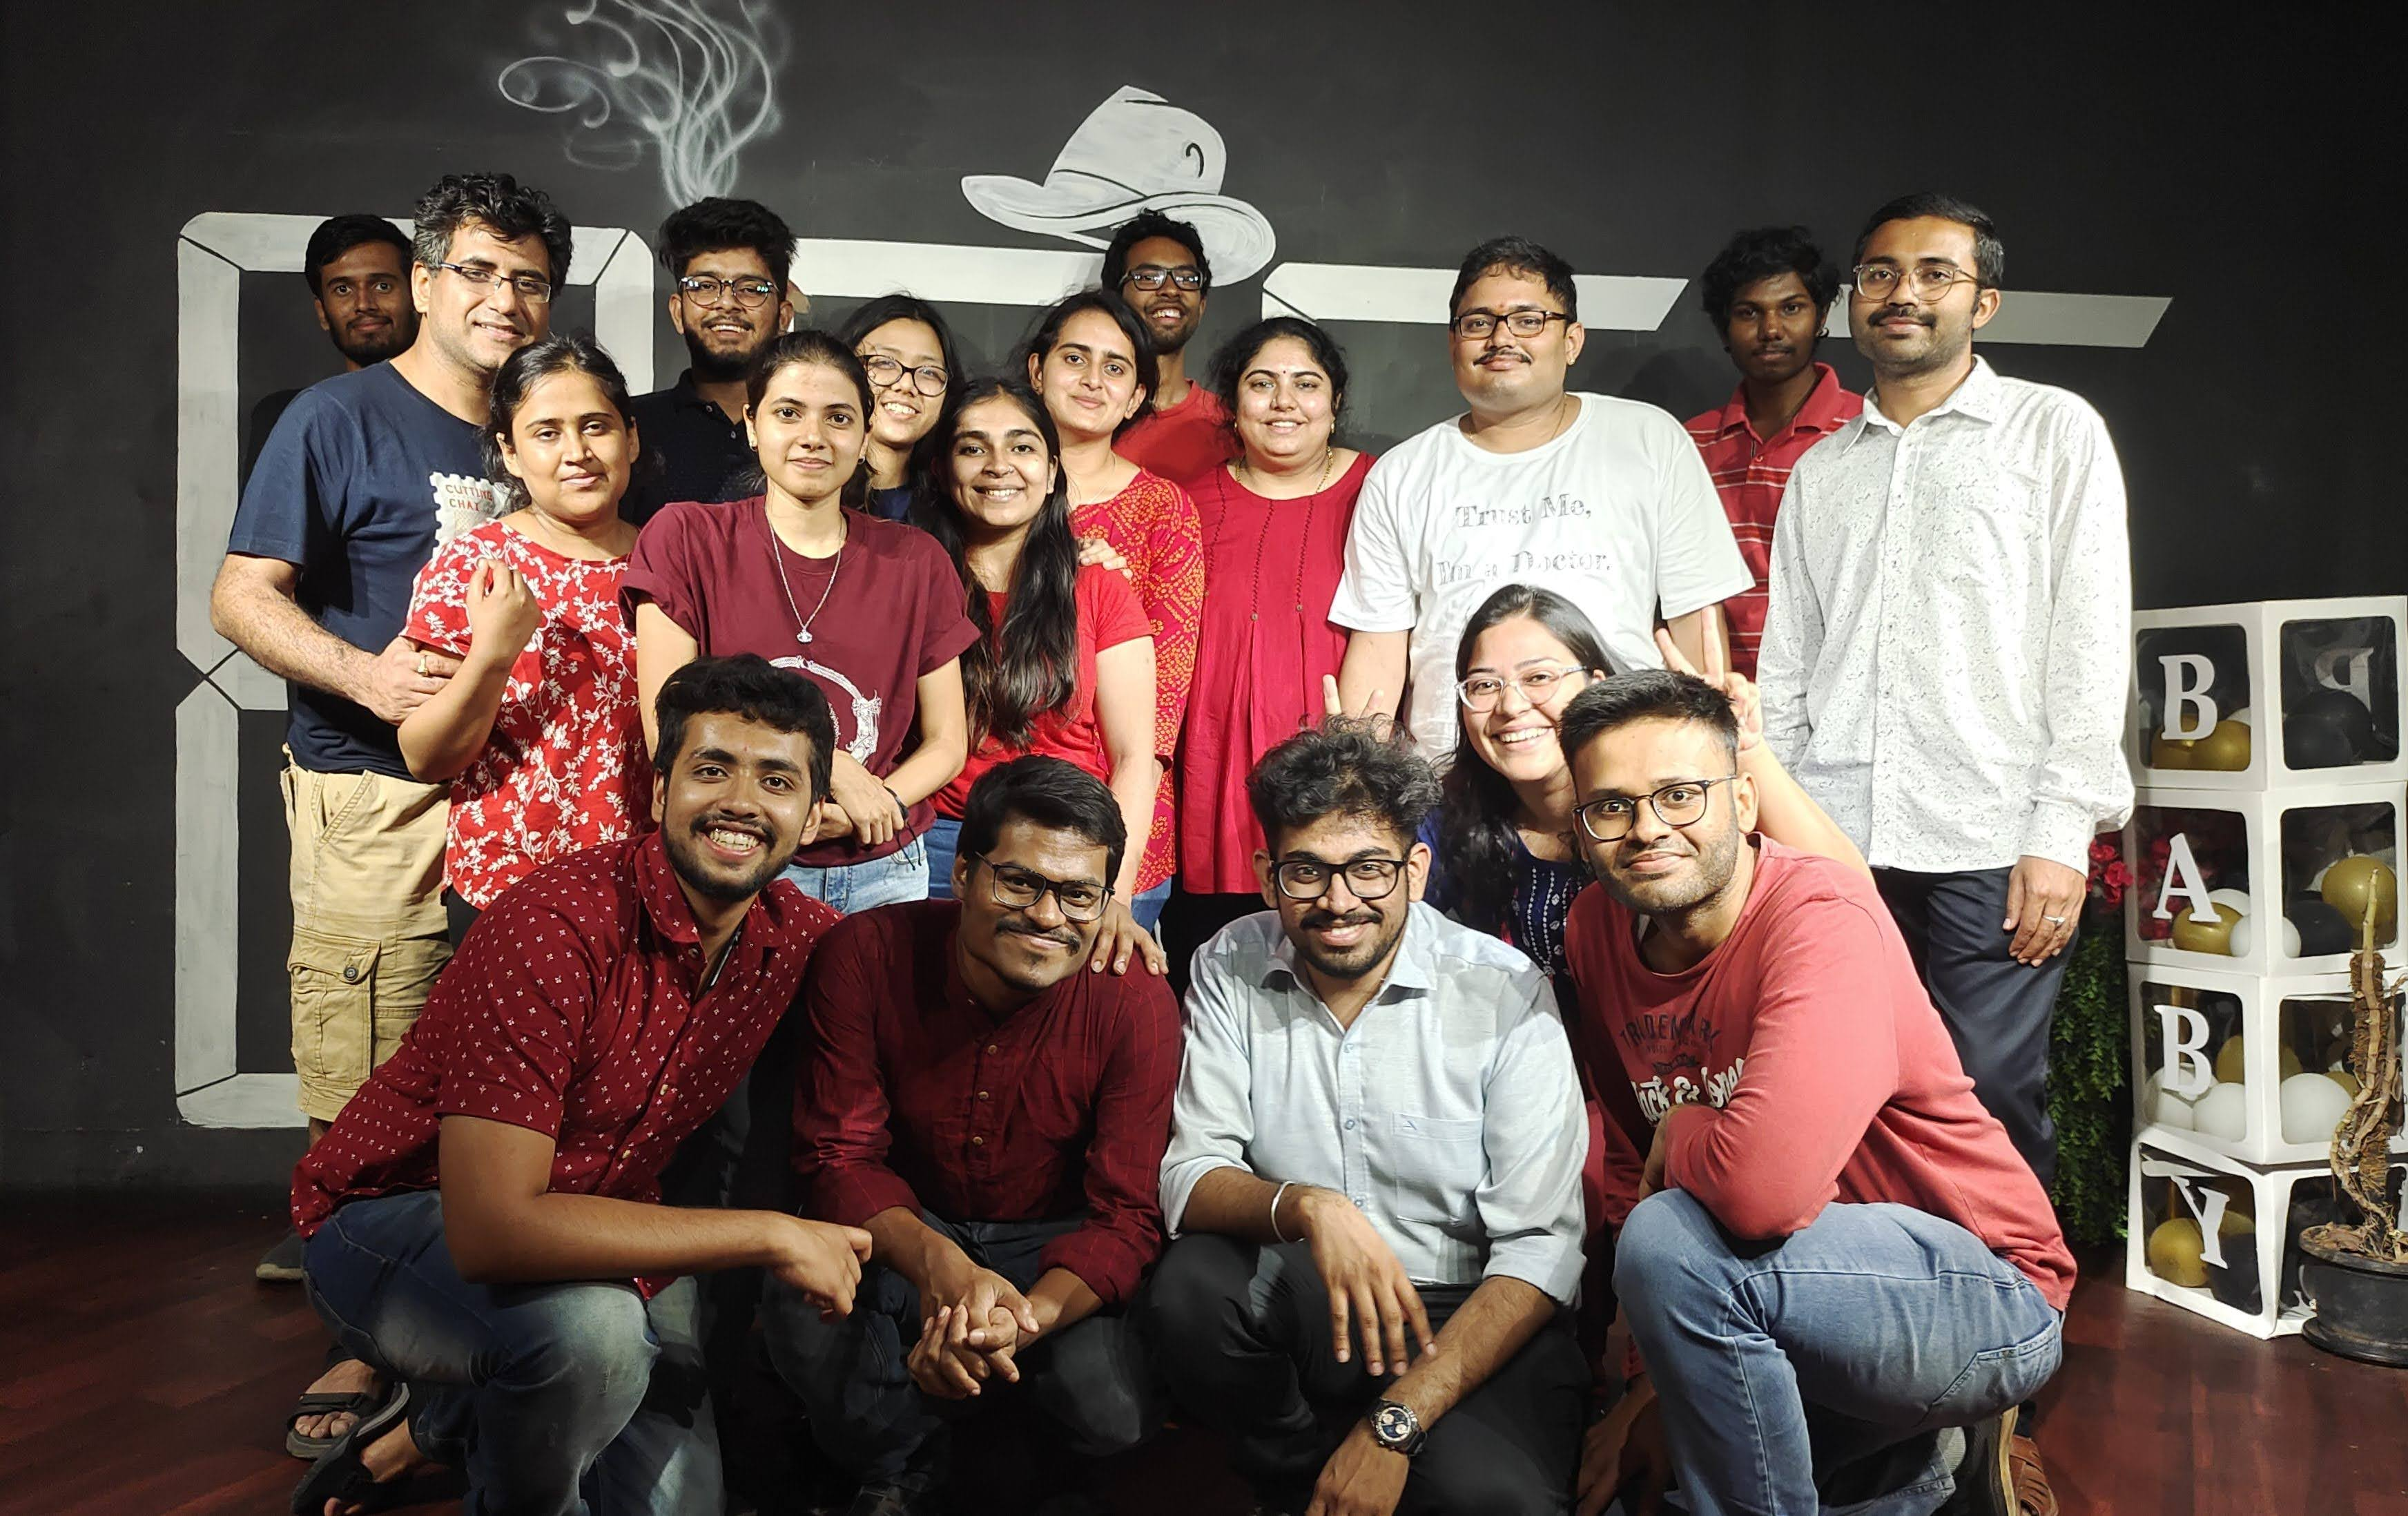
\includegraphics[width=\textwidth]{CSBLab}
        \end{figure}
        \begin{figure}
            
\includegraphics[width=0.2\textwidth]{PMRF_Logo}
        \end{figure}
        \end{column}
        \begin{column}{0.35\textwidth}
        \center{\Huge Thank You}
        \end{column}
    \end{columns}

    \end{frame}

    \begin{frame}[allowframebreaks]
        \printbibliography
    \end{frame}

\end{document}

